\documentclass[11pt,a4paper,openany,leqno]{article}

\textwidth=160mm \textheight=260mm \hoffset=-18mm \voffset=-30mm
\setcounter{page}{1}
			\usepackage[magyar]{babel}
			\usepackage[utf8]{inputenc}
			\usepackage[T1]{fontenc}
			\usepackage{indentfirst}
			\usepackage{amsmath,esint}
			\usepackage{amssymb}
%			\usepackage{eufrak}
			\usepackage{psfrag}
			\usepackage{tabularx}
			\usepackage{graphicx}
			\usepackage{wrapfig}	
			\usepackage{hyperref}
			\usepackage{multicol}	
									
			\frenchspacing
			\allowhyphens

\tolerance=2000
\hbadness=2000
\vbadness=10000
\overfullrule=0pt




\begin{document}
\section{Ohm-törvény}
\subsection{Elméleti Fizikai Példatár II./ 4.3. feladat}



Négyzetháló $n^2$ (egyforma homogén vezetőhuzalból készült) számú sejtből áll. Mindegyik huzal ellenállása $r$. Az áram a rács egyik csúcspontjából indul ki és a szemközti csúcsba megy. Határozzuk meg az egész rács $R$ ellenállását az $n = 2, 3$ esetekben!

\medskip
$a)$ $n = 2$

\medskip
$a)$ $n = 3$


\begin{flushright} {Feladatot kidolgozta: {\it Z2R8XS}} \end{flushright}

\vspace{0.5cm}

\textbf{Megoldás}\\
\indent
Egy-egy huzal darabkát felfoghatunk úgy, mint egy-egy ellenállás. Két csomópont közti huzal darabka úgy viselkedik, mint egy ellenállás, ami tökéletesen vezető drótokkal van kötve a két csomóponthoz.\\ \indent
Soros kapcsolás esetén : $R_e = R_1 + R_2$ \\ \indent
Párhuzamos kapcsolás esetén : $\frac{1}{R_e} = \frac{1}{R_1} + \frac{1}{R_2}$ \\ \indent
Csillag delta kapcsolás esetén : \\
\smallskip
\indent
$\Delta - Y$
$$ R_A = \frac{R_1 \cdot R_2}{R_1 + R_2 + R_3} $$
$$ R_B = \frac{R_1 \cdot R_3}{R_1 + R_2 + R_3} $$
$$ R_C = \frac{R_2 \cdot R_3}{R_1 + R_2 + R_3} $$ \indent
ahol $A$, $B$ és $C$ pontok a "kimeneti pontok". Az adott pontnak megfelelő ellenállás a pontba "befutó" két ellenállás szorzatával arányos. Tehát az $A$ pontba $R_1$ és $R_2$ ellenállás "fut be".\\ \indent
\smallskip
$Y- \Delta$
$$ R_1 = \frac{R_A \cdot R_B}{R_C} + R_A + R_B $$
$$ R_2 = \frac{R_A \cdot R_C}{R_B} + R_A + R_C $$
$$ R_3 = \frac{R_B \cdot R_C}{R_A} + R_B + R_C $$ \indent
A következőkben csillag alatt $Y$ alakú kapcsolást, delta alatt $\Delta$ alakú kapcsolást értek, csillag-delta kapcsolás alatt pedig ezen esetek gyűjtőnevét.
\medskip



\textbf{a) n=2}
\medskip

\indent
Itt az alábbi módon helyezkednek el az ellenállások.\\

\begin{figure}[h!]
\centering
  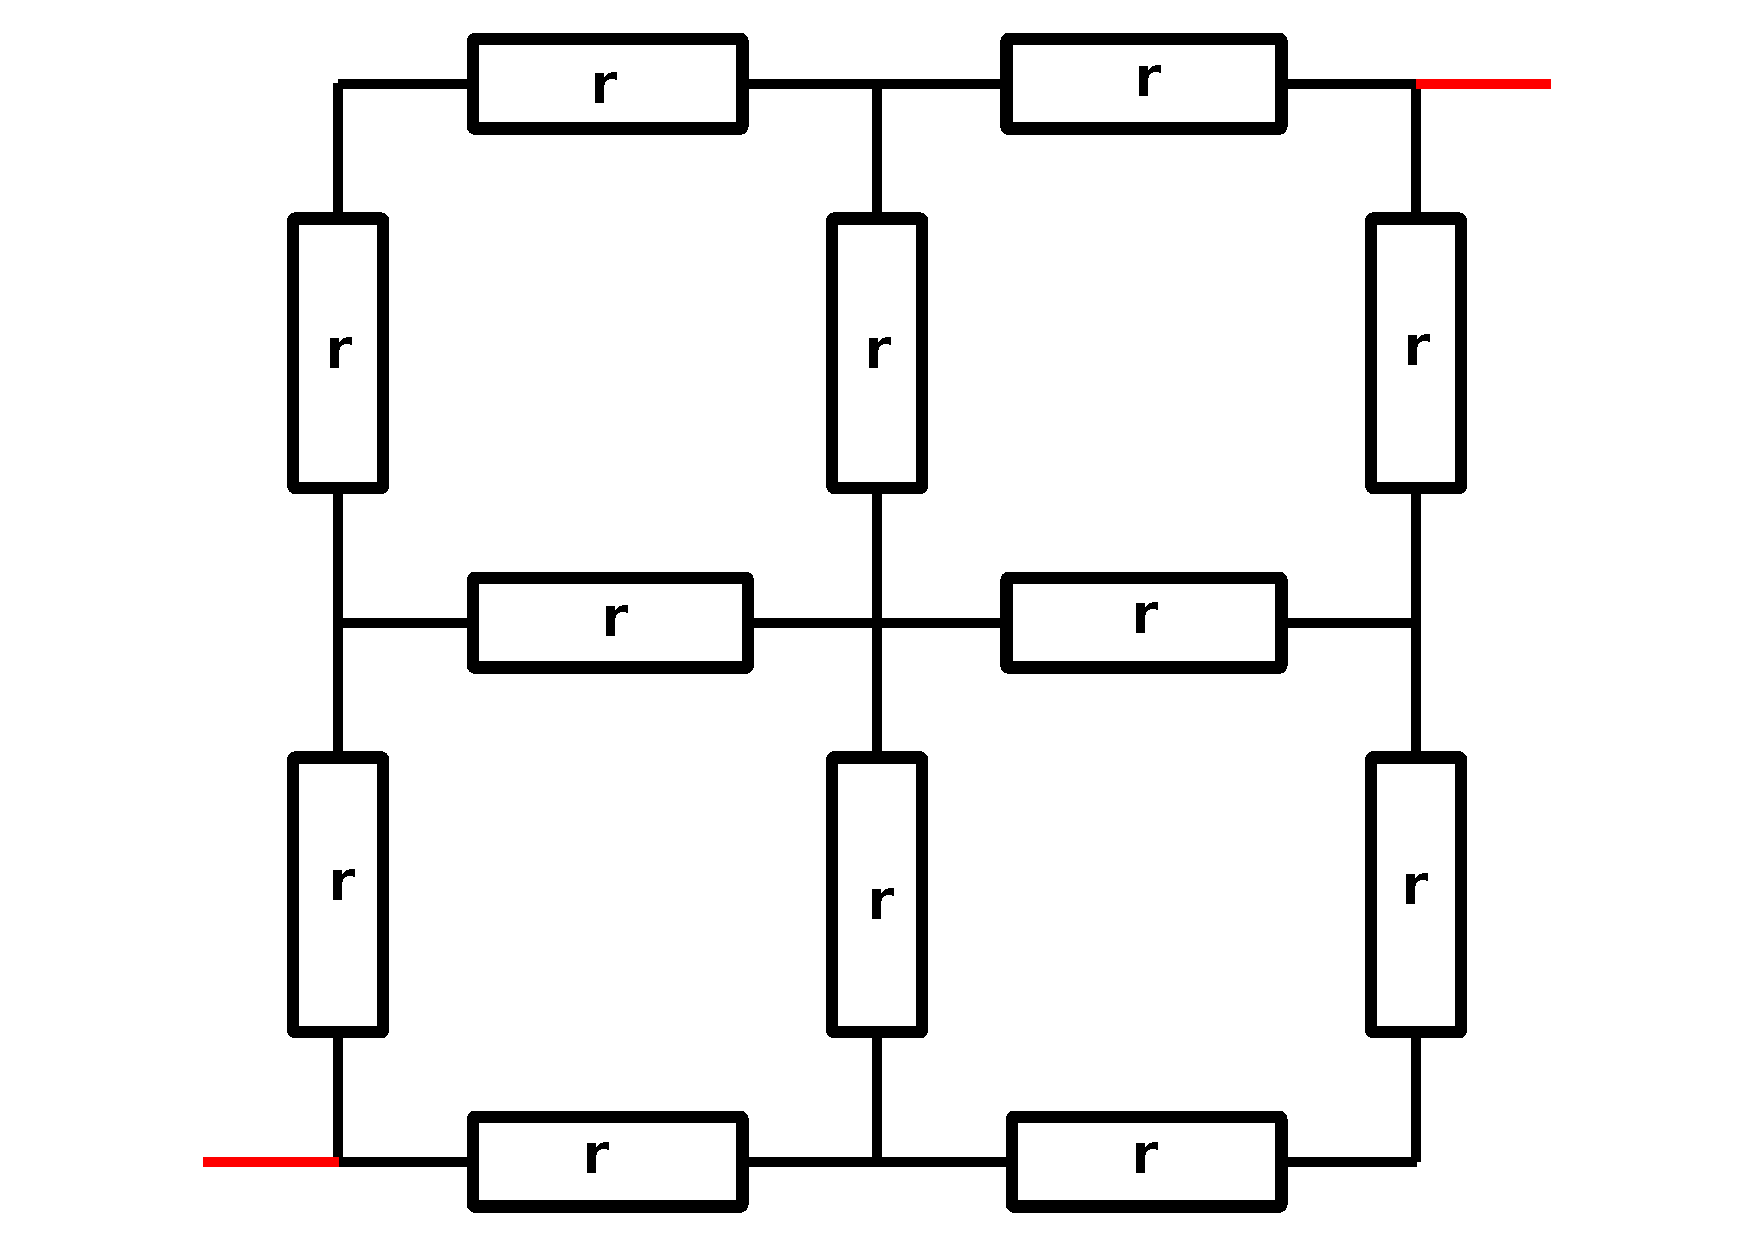
\includegraphics[width=100mm,scale=0.5]{grid_2_1.pdf}
  \caption{2x2 rács}
  \label{}
\end{figure}
\newpage
\indent
Látható, hogy a jobb alsó és a bal felső sarokban két-két ellenállás sorosan van kapcsolva. Ezek összevonhatóak összeadással.\\

\begin{figure}[h!]
\centering
  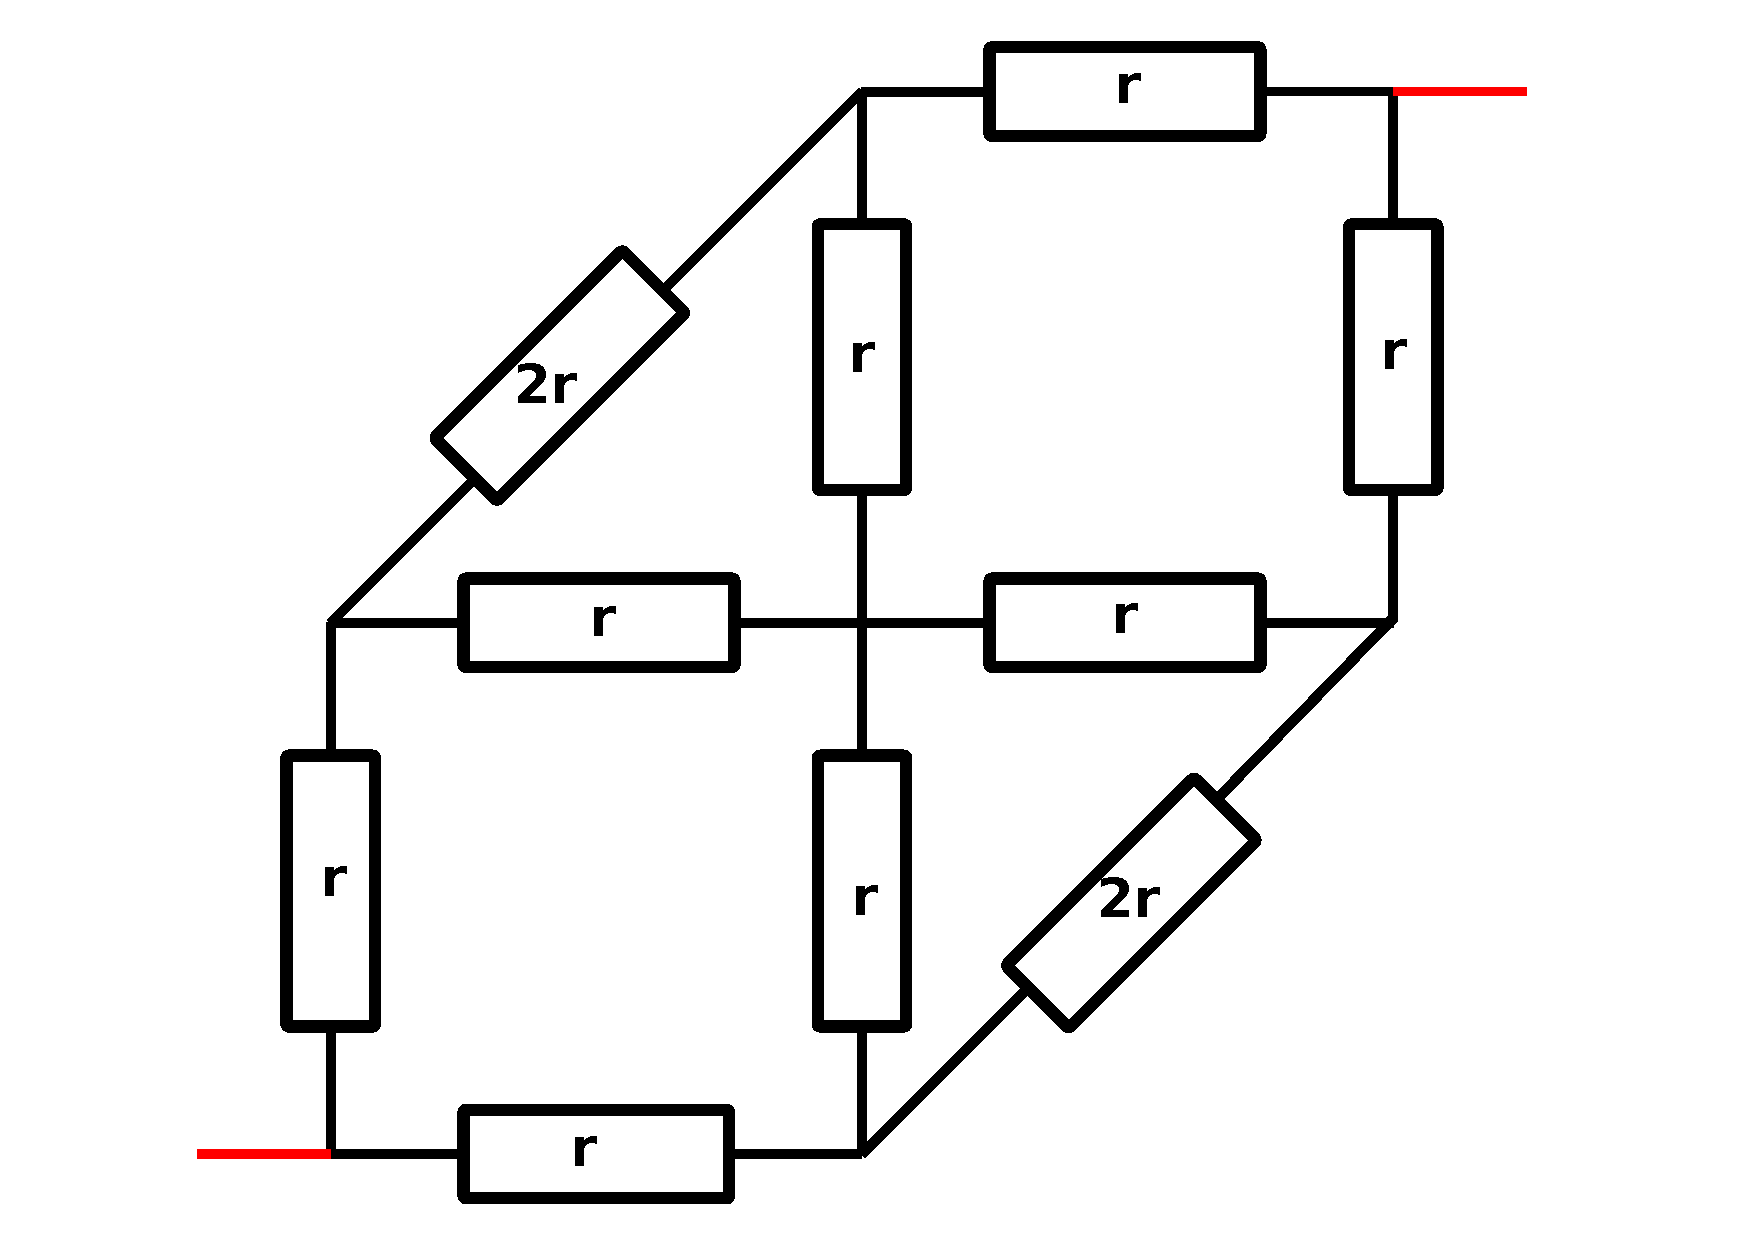
\includegraphics[width=100mm,scale=0.5]{grid_2_2.pdf}
  \caption{Sarkok egyszerűsítése}
  \label{}
\end{figure}
\newpage
\indent
Itt a jobb alsó és a bal felső sarokban találkozunk egy-egy csillag-delta alakú kapcsolással. E két csillag-delta találkozik középen. A rendszer szerencsére szimmetrikus. \\

\begin{figure}[h!]
\centering
  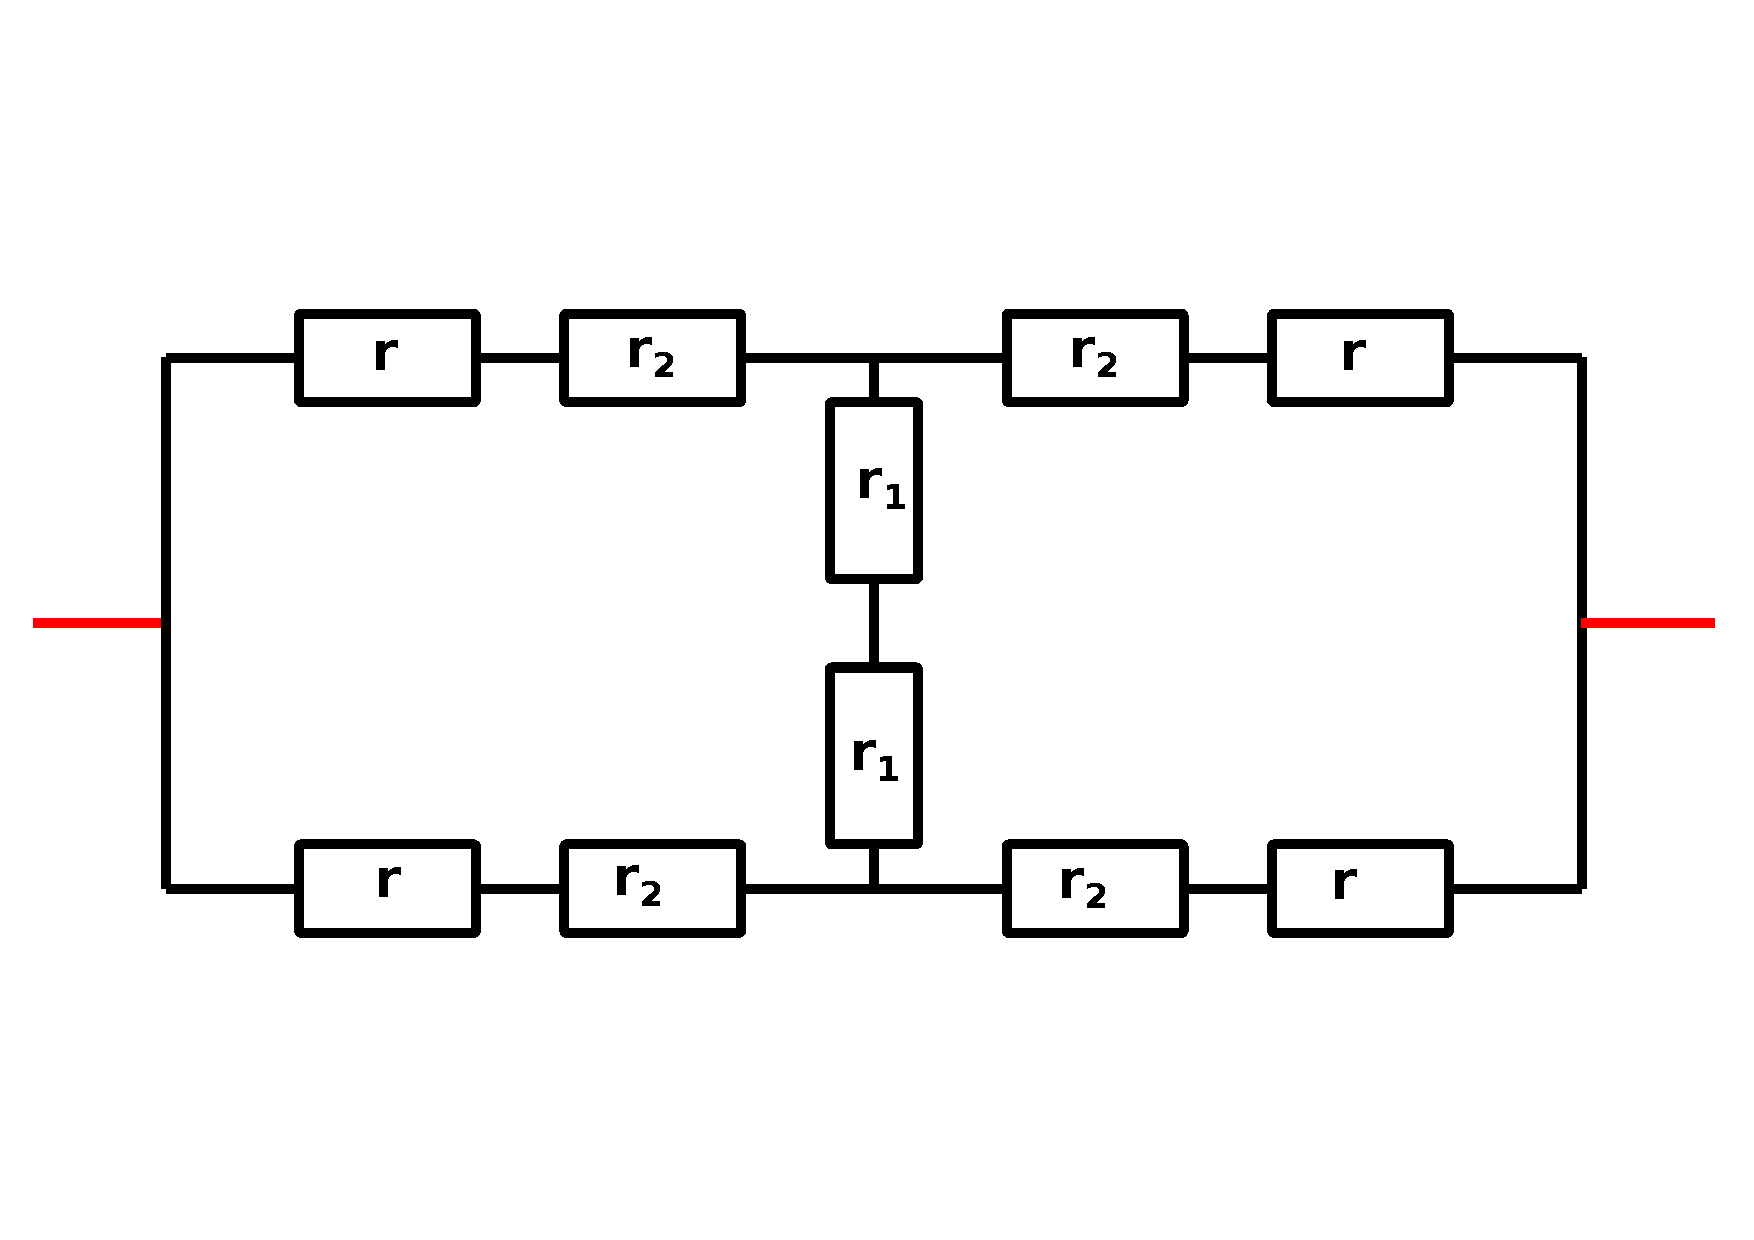
\includegraphics[width=100mm,scale=0.5]{grid_2_3.pdf}
  \caption{Csillag-delta kapcsolások a sarkokban}
  \label{}
\end{figure}
$$ r_1 = \frac{r^2}{4r} = \frac{1}{4}r $$
$$ r_2 = \frac{2r^2}{4r} = \frac{1}{2}r $$
\newpage
\begin{figure}[h!]
\centering
  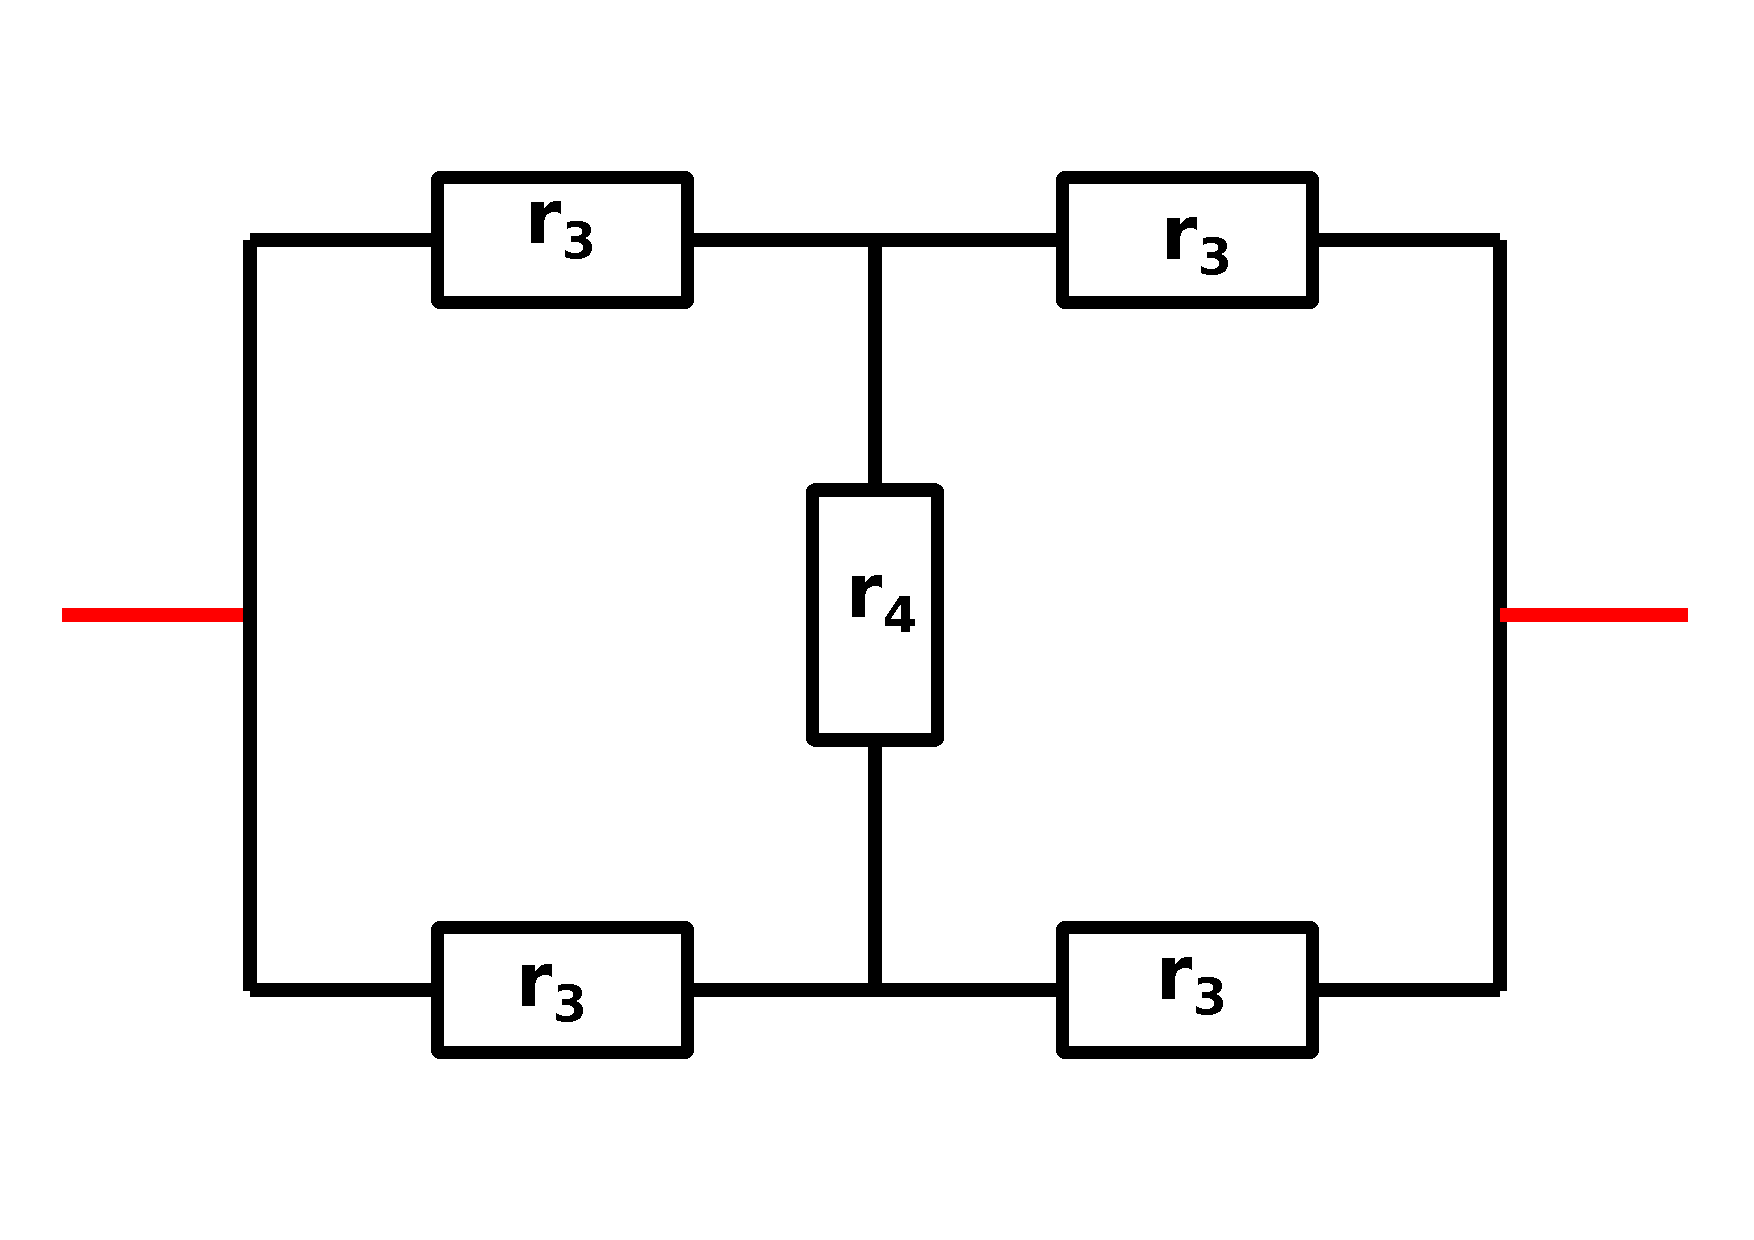
\includegraphics[width=100mm,scale=0.5]{grid_2_4.pdf}
  \caption{Összevonások}
  \label{}
\end{figure}
$$ r_3 = r + r_2 = \frac{3}{2}r $$
$$ r_4 = r_1 + r_1 = \frac{1}{2}r $$
\indent
A felső kettő és a középső ellenállás csillag delta kapcsolást képez, ez is átalakítható. Mivel átalakítás után a háromszög két csúcsát nem választja el semmi a kimeneti és a bemeneti kábeltől, ezért le lehet húzni ez a két pontot közvetlenül a piros vonalakhoz, ekvipotenciális pontokkal kábel mentén ez megtehető.\\

\begin{figure}[h!]
\centering
  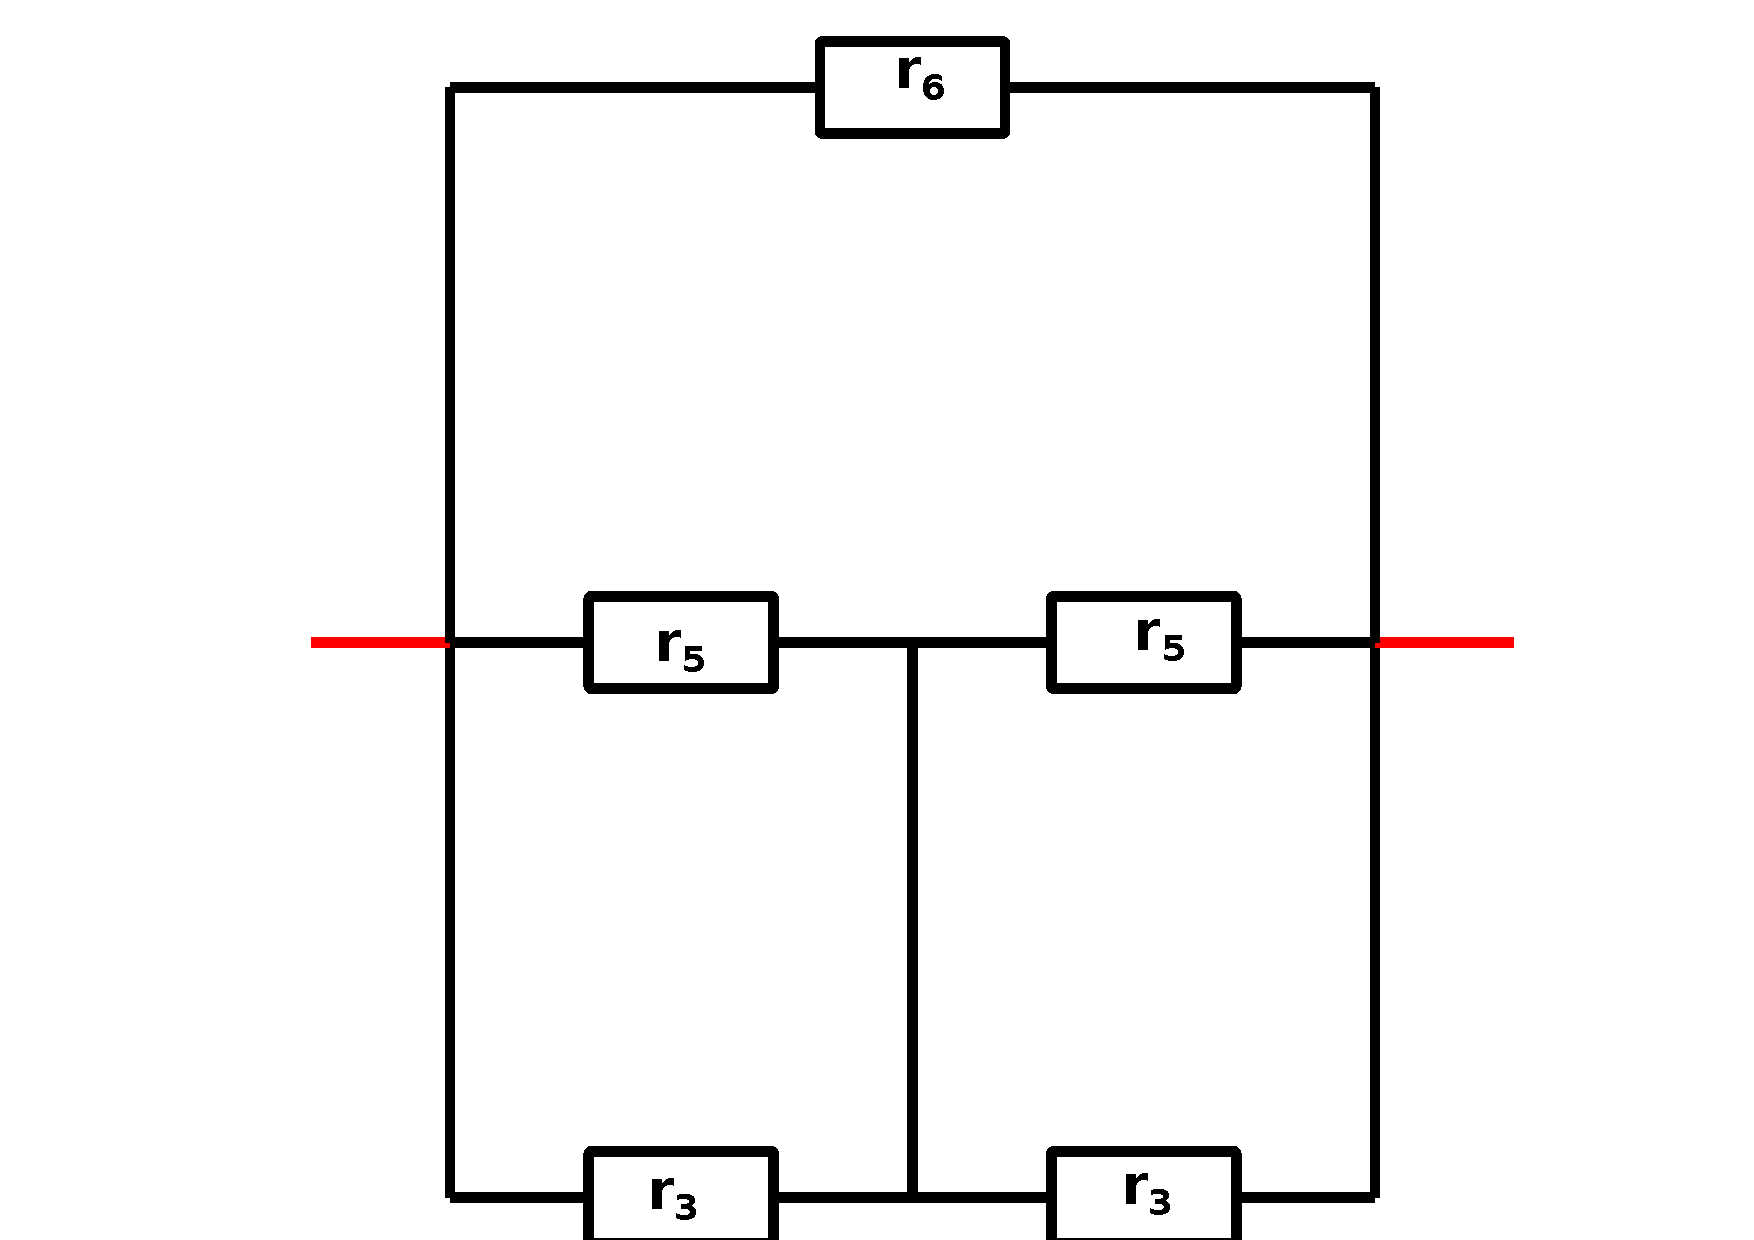
\includegraphics[width=100mm,scale=0.5]{grid_2_5.pdf}
  \caption{Csillag-delta átalakítás utáni széthúzása}
  \label{}
\end{figure}
Az alsó kettő marad $r_3$, a többiek:
$$ r_5 = \frac{r_3 \cdot r_4}{r_3} + r_3 + r_4 = \frac{1}{2}r + \frac{3}{2}r + \frac{1}{2}r = \frac{5}{2}r $$
$$ r_6 = \frac{r_3 \cdot r_3}{r_4} + r_3 + r_3 = \frac{9}{2}r + \frac{6}{2}r = \frac{15}{2}r$$


Bár a középső kábelen nem folyik áram, egy rövidzárnak tekinthető két pont között, így nem hagyható el. A helyes átalakítás az lenne, hogy széthúzzunk két klasszikus párhuzamos kapcsolásra.\\

\begin{figure}[h!]
\centering
  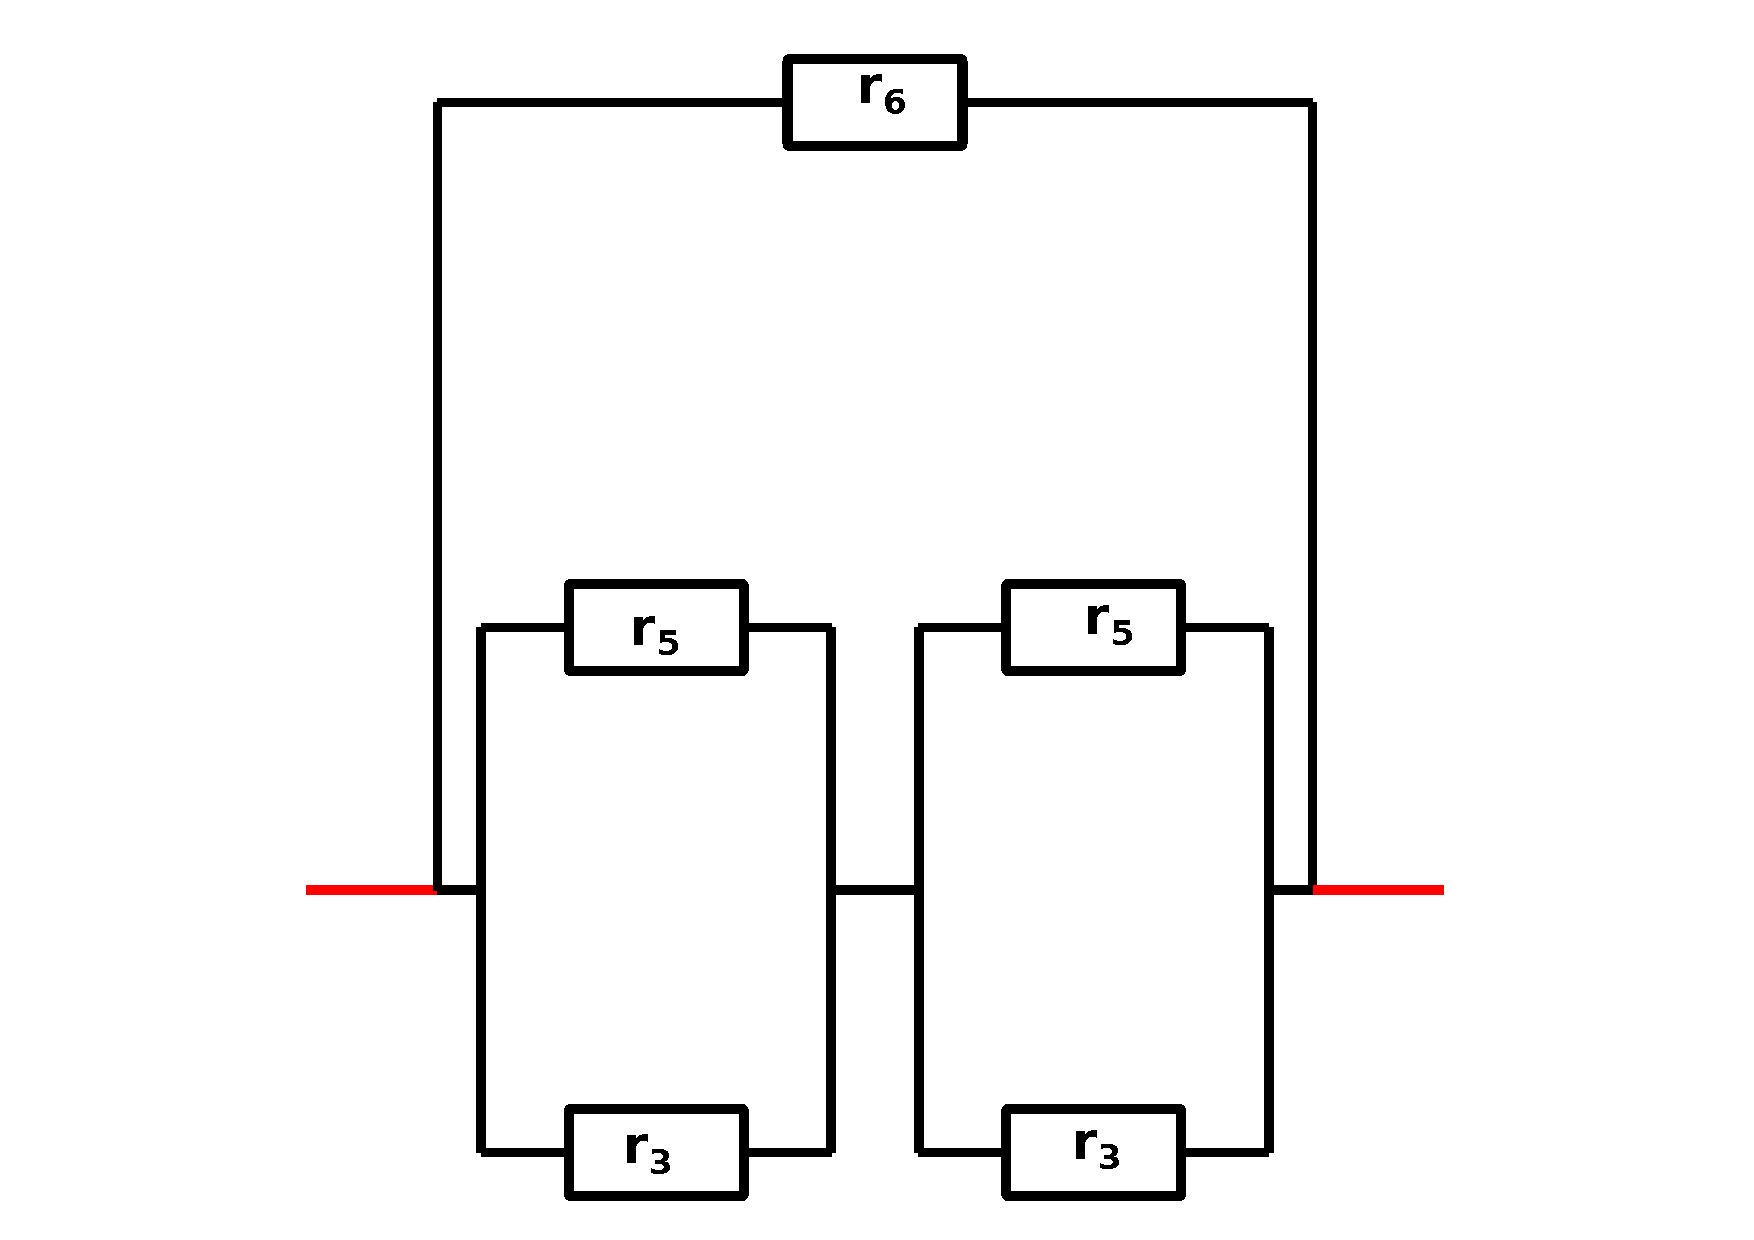
\includegraphics[width=150mm,scale=0.5]{grid_2_6.pdf}
  \caption{Párhuzamos kapcsolásokra való bontás}
  \label{}
\end{figure}
\indent
Az lenti két párhuzamos kapcsolás külön-külön átalakítható. Átalakítás után e két párhuzamos kapcsolás eredője sorosan lesz kötve, így gond nélkül összeadhatóak. Mindezek után már csak két ellenállás marad párhuzamosan kötve.\\
$$ \frac{1}{r_7} = \frac{1}{r_3} + \frac{1}{r_5} = \frac{r_3 + r_5}{r_3 \cdot r_5} = \frac{4}{\frac{15}{4}r} $$
$$ r_7 = \frac{15}{16}r $$
$$ r_8 = 2r_7 = \frac{15}{8}r $$
$$ \frac{1}{R} = \frac{1}{r_8} + \frac{1}{r_6} = \frac{r_6 + r_8}{r_6 \cdot r_8} = \frac{\frac{75}{8}}{\frac{225}{16}r} = \frac{10}{15r} = \frac{2}{3r} $$
$$ R = \frac{3}{2}r $$


\newpage
\textbf{b) n = 3}

Itt az alábbi módon helyezkednek el az ellenállások.\\

\begin{figure}[h!]
\centering
  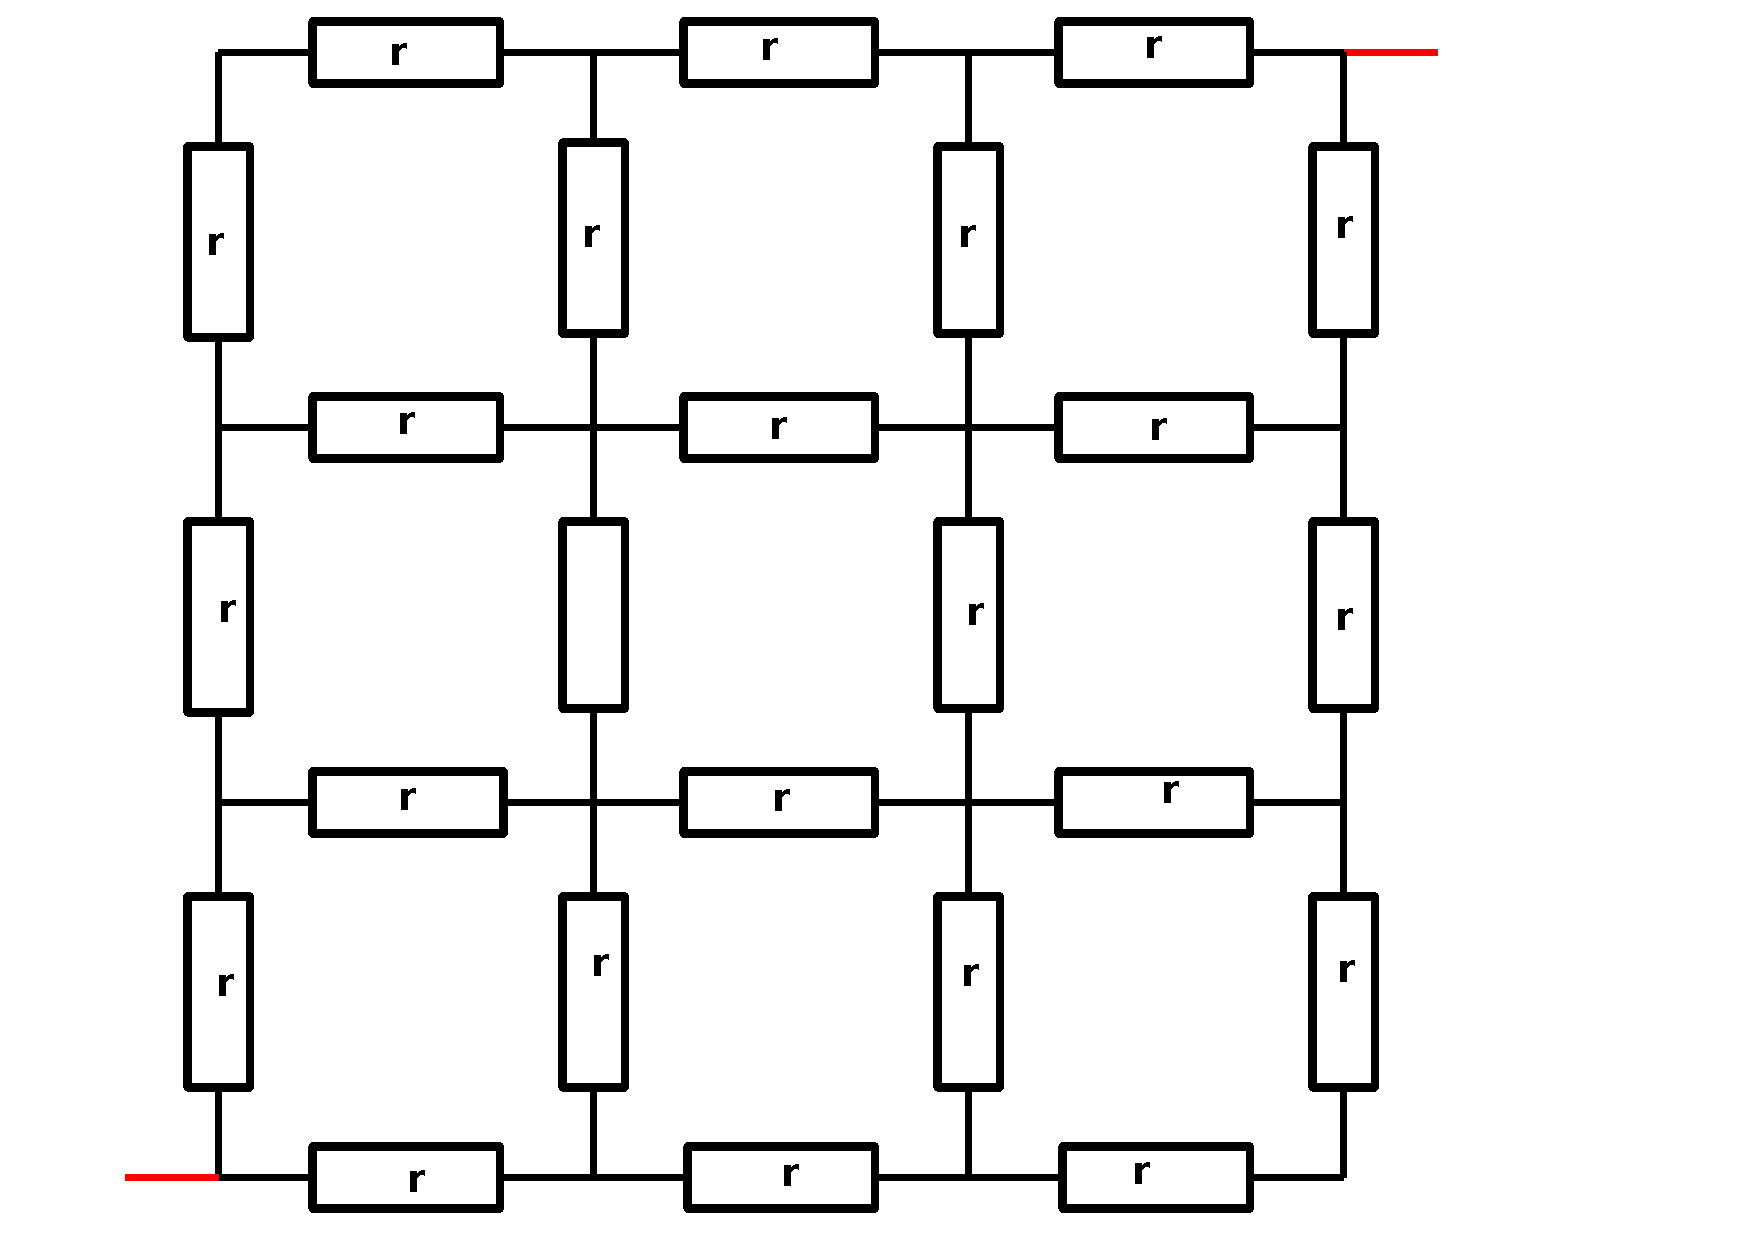
\includegraphics[width=150mm,scale=0.5]{grid_3_1.pdf}
  \caption{3x3 grid}
  \label{}
\end{figure}
 \newpage
Hasonlóan a jobb alsó és a bal felső sarokban két-két ellenállás sorosan van kapcsolva. Ezek összevonhatóak összeadással.\\

\begin{figure}[h!]
\centering
  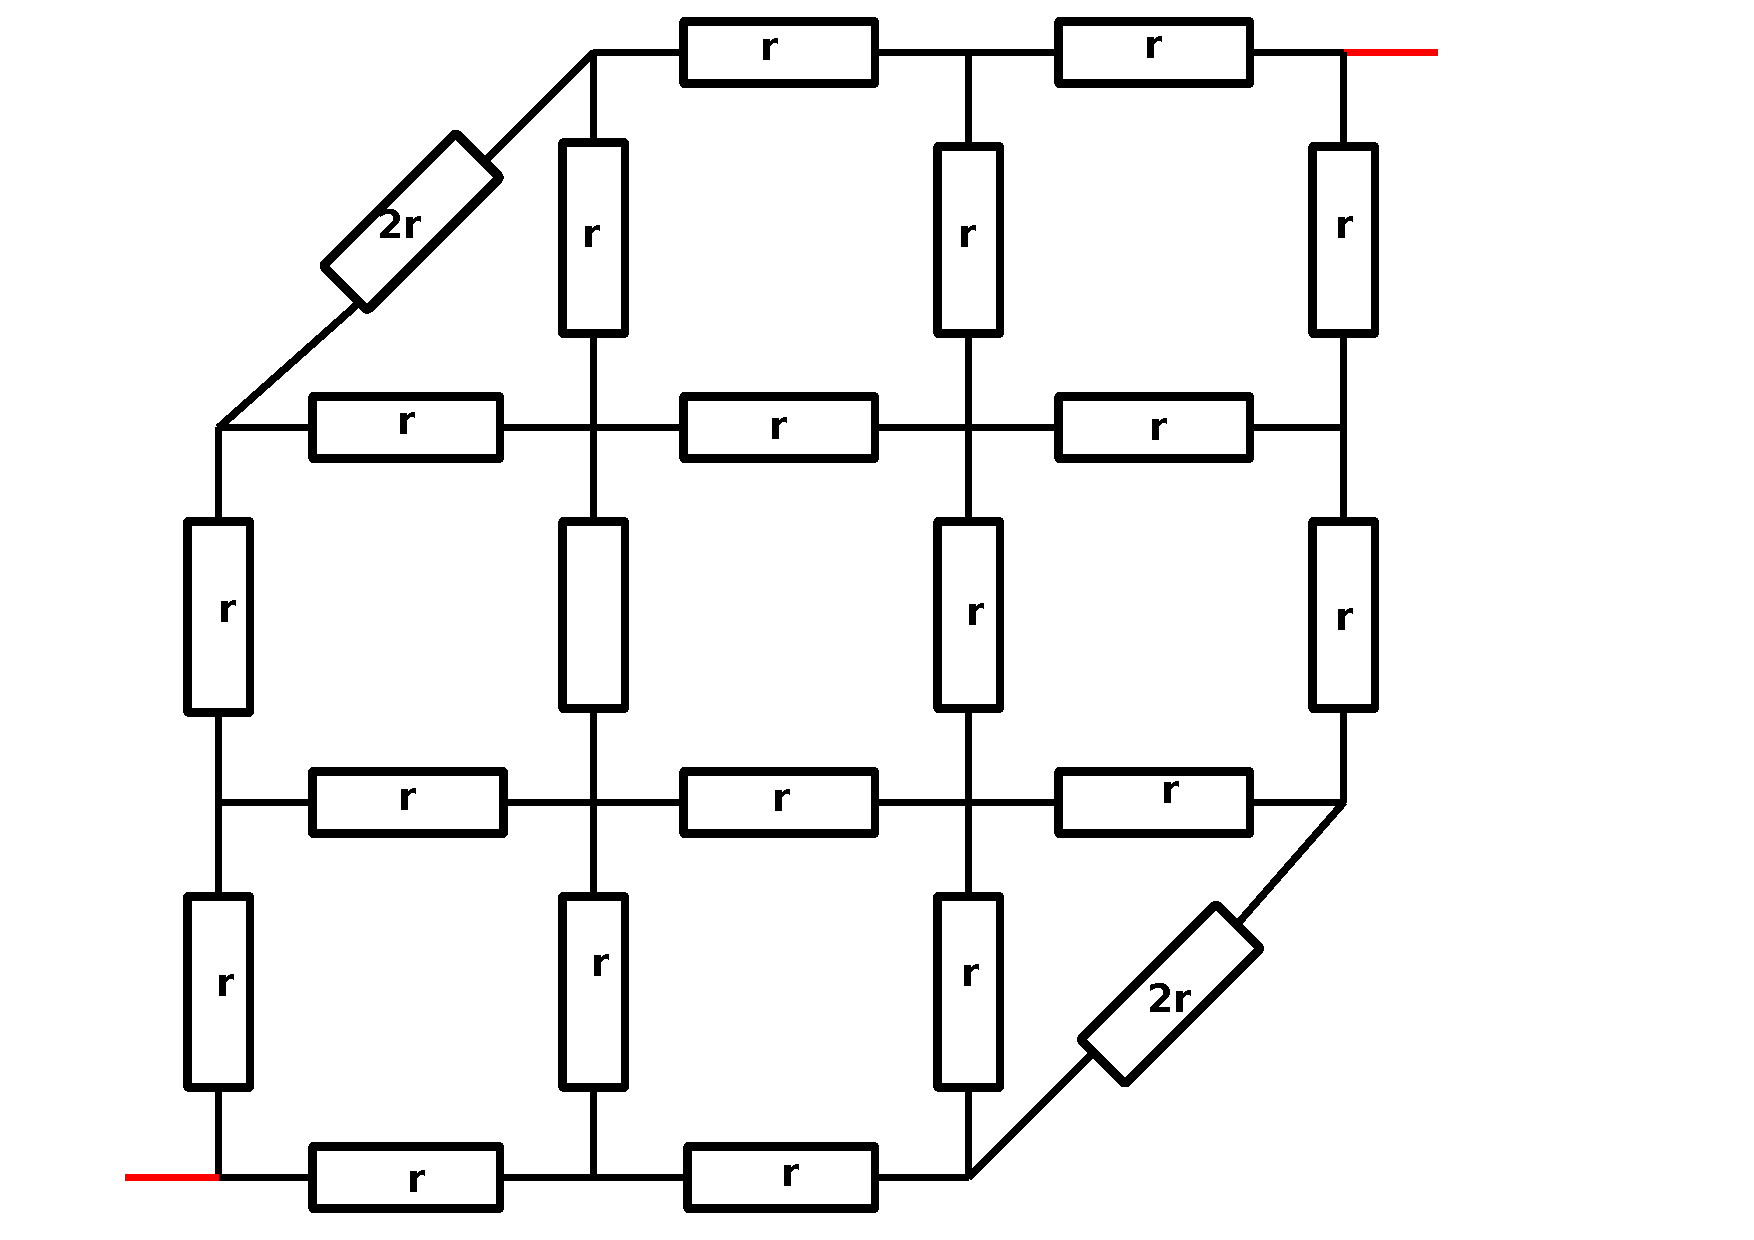
\includegraphics[width=150mm,scale=0.5]{grid_3_2.pdf}
  \caption{Sarkok egyszerűsítése}
  \label{}
\end{figure}
\newpage




E két sarokban végezhető csillag delta kapcsolásos átalakítás.\\

\begin{figure}[h!]
\centering
  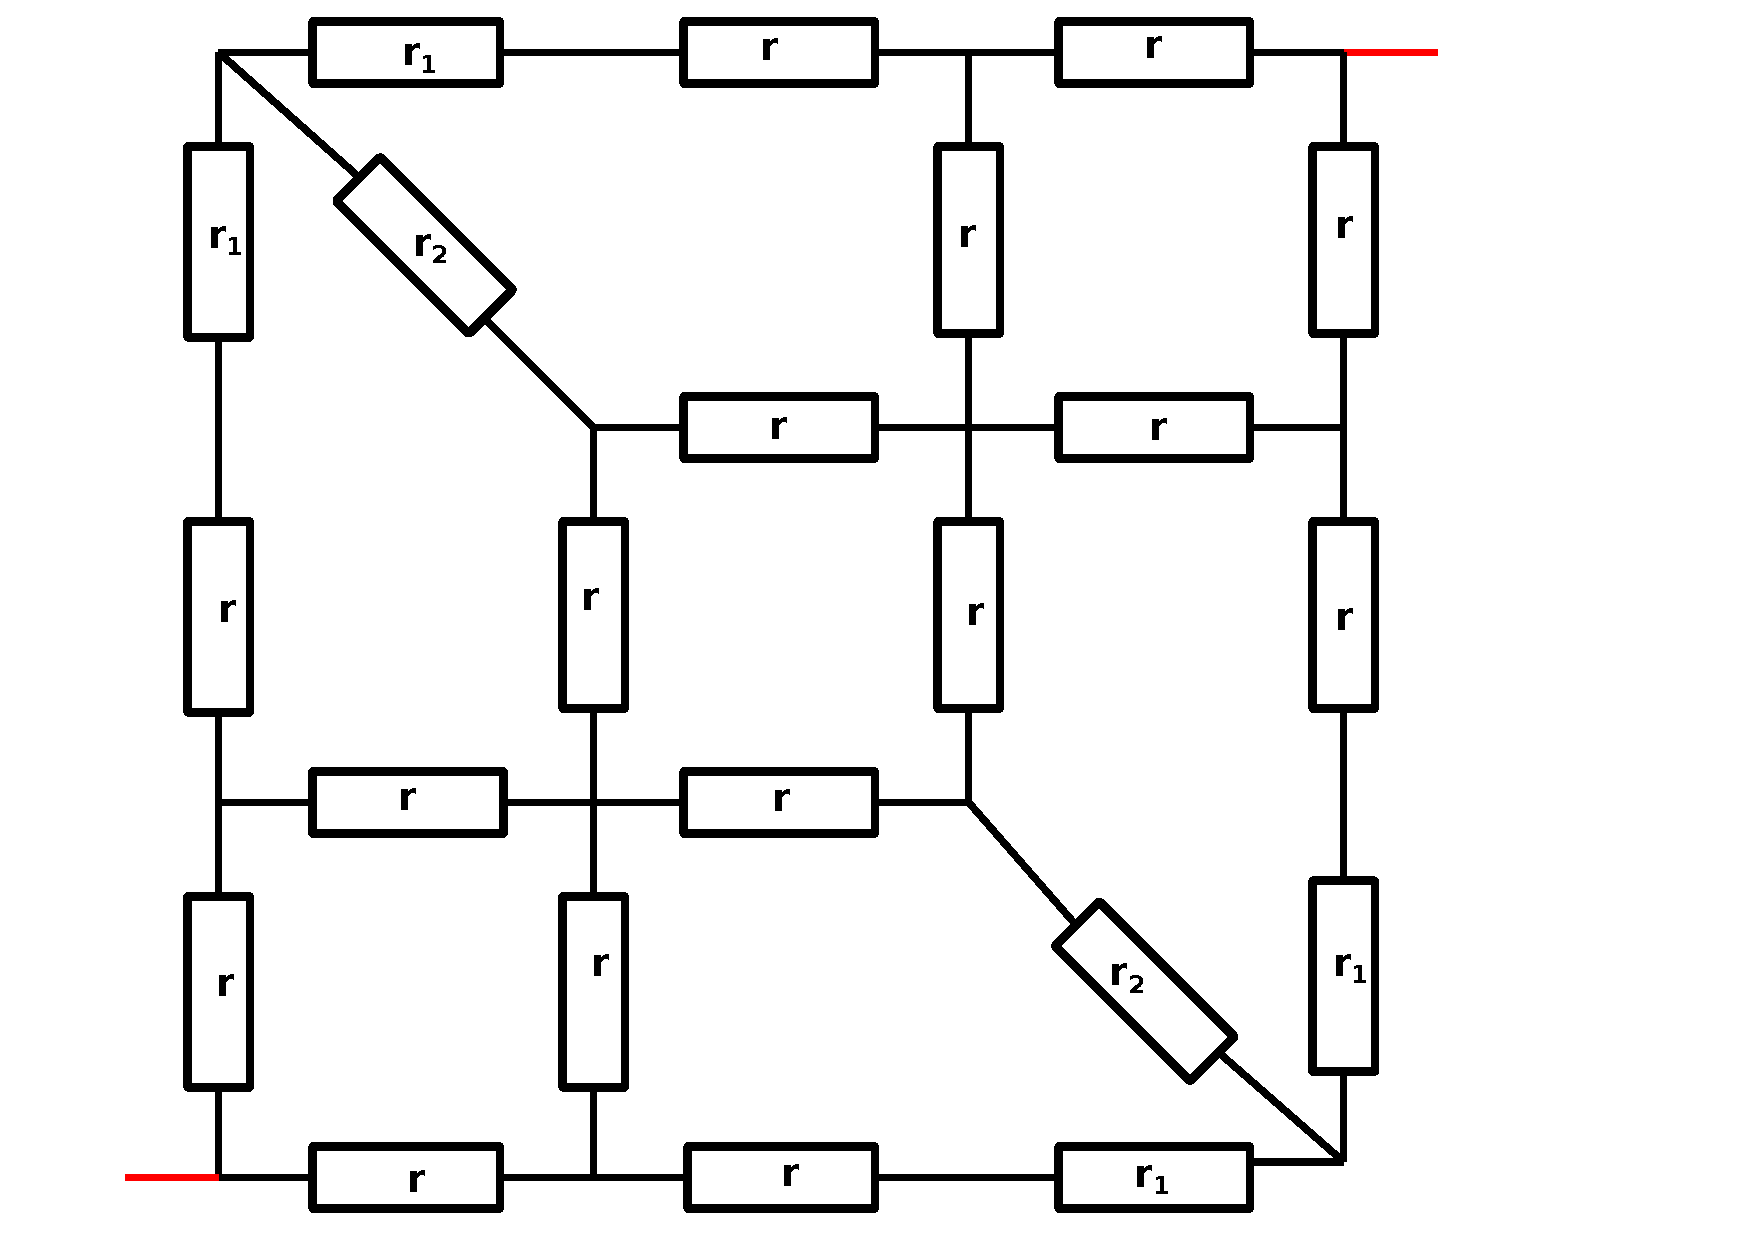
\includegraphics[width=150mm,scale=0.5]{grid_3_3.pdf}
  \caption{Csillag-delta kapcsolások a sarkokban}
  \label{}
\end{figure}
$$ r_1 = \frac{2r}{4} = \frac{1}{2} r $$
$$ r_2 = \frac{r}{4} = \frac{1}{4} r $$
\newpage

Kapunk négy pár sorosan kapcsolt ellenállást, melyek csak arra várnak, hogy összeadják őket.\\

\begin{figure}[h!]
\centering
  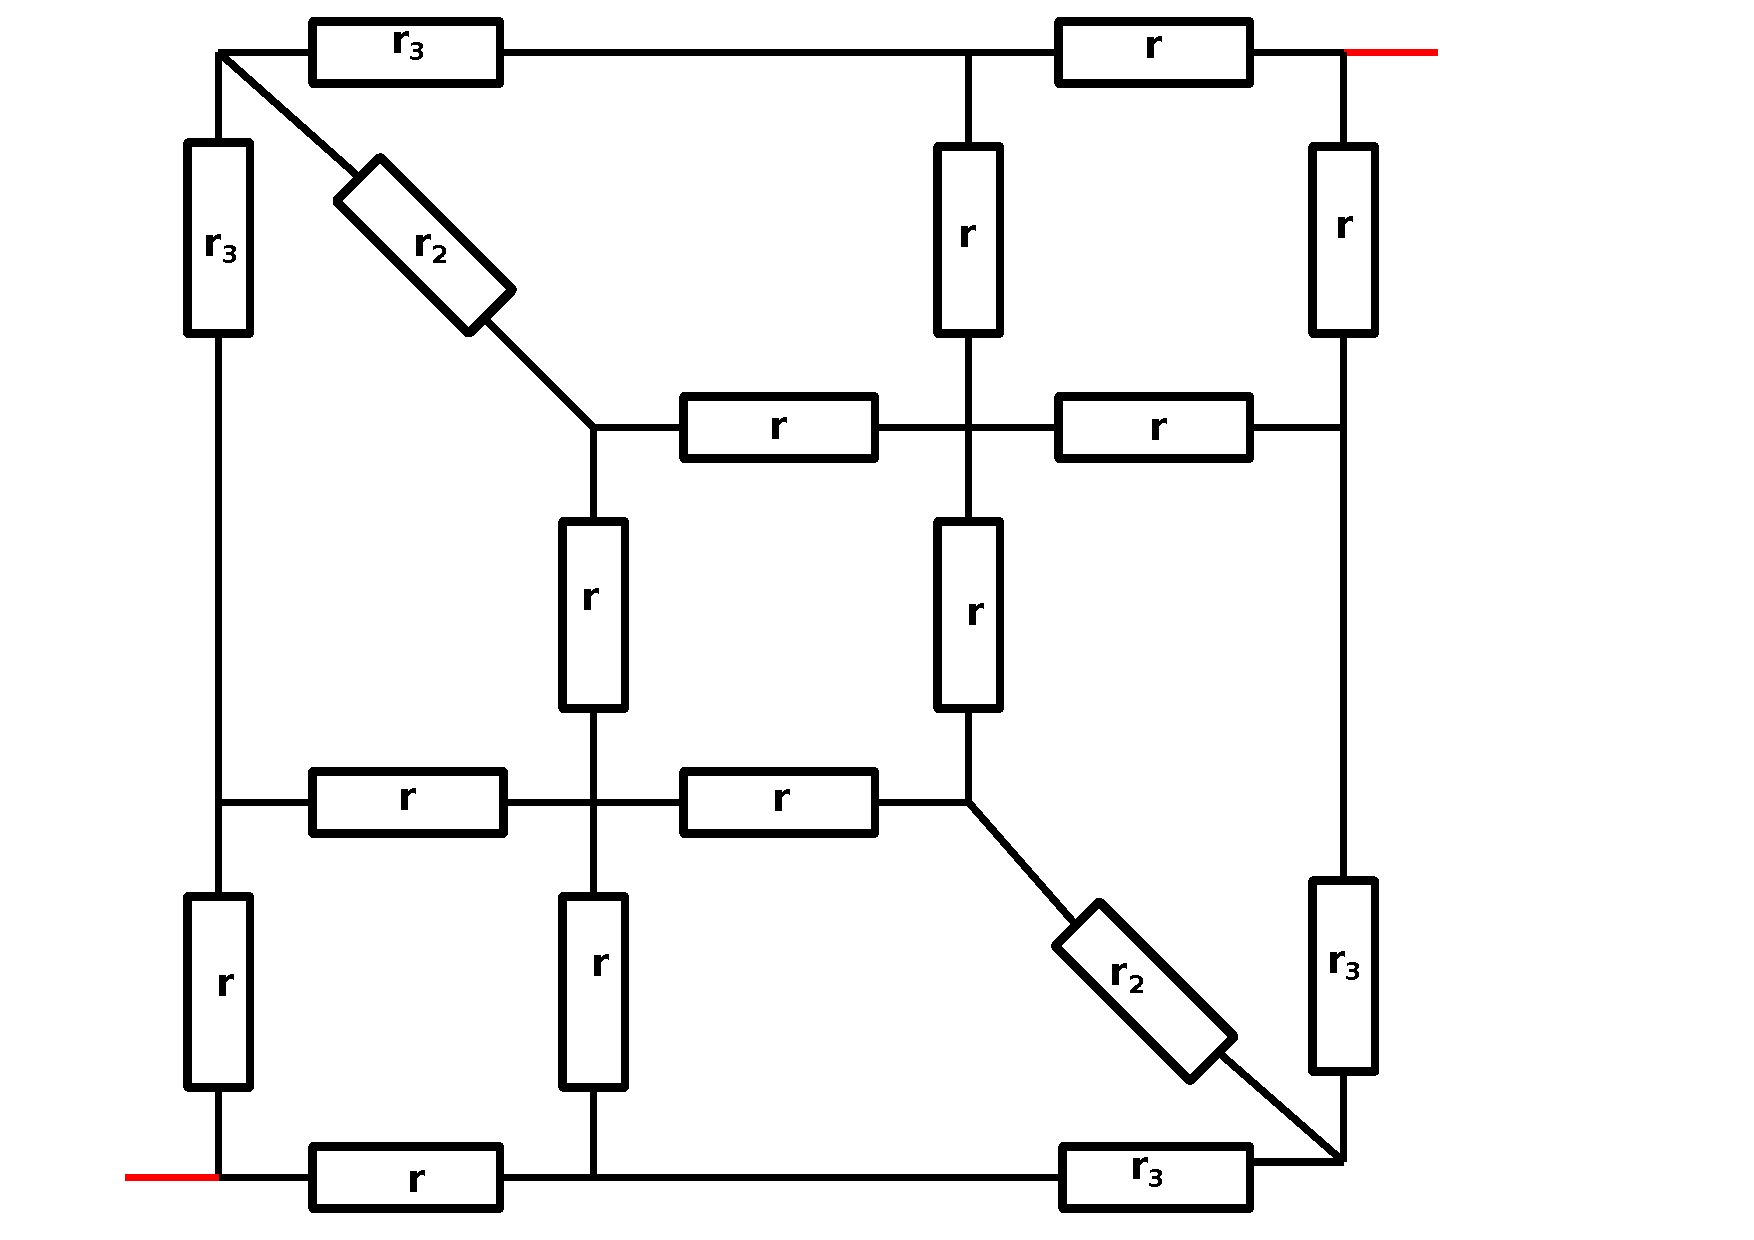
\includegraphics[width=150mm,scale=0.5]{grid_3_3a.pdf}
  \caption{Összevonások}
  \label{}
\end{figure}

$$ r_3 = r + r_1 = \frac{3}{2} r $$


Az ábra hasonlóan néz ki, már pár ellenállást bekebeleztek a csillag delták. \\
\newpage
Középen, ferde sávban felbukkan négy csillag delta. \\

\begin{figure}[h!]
\centering
  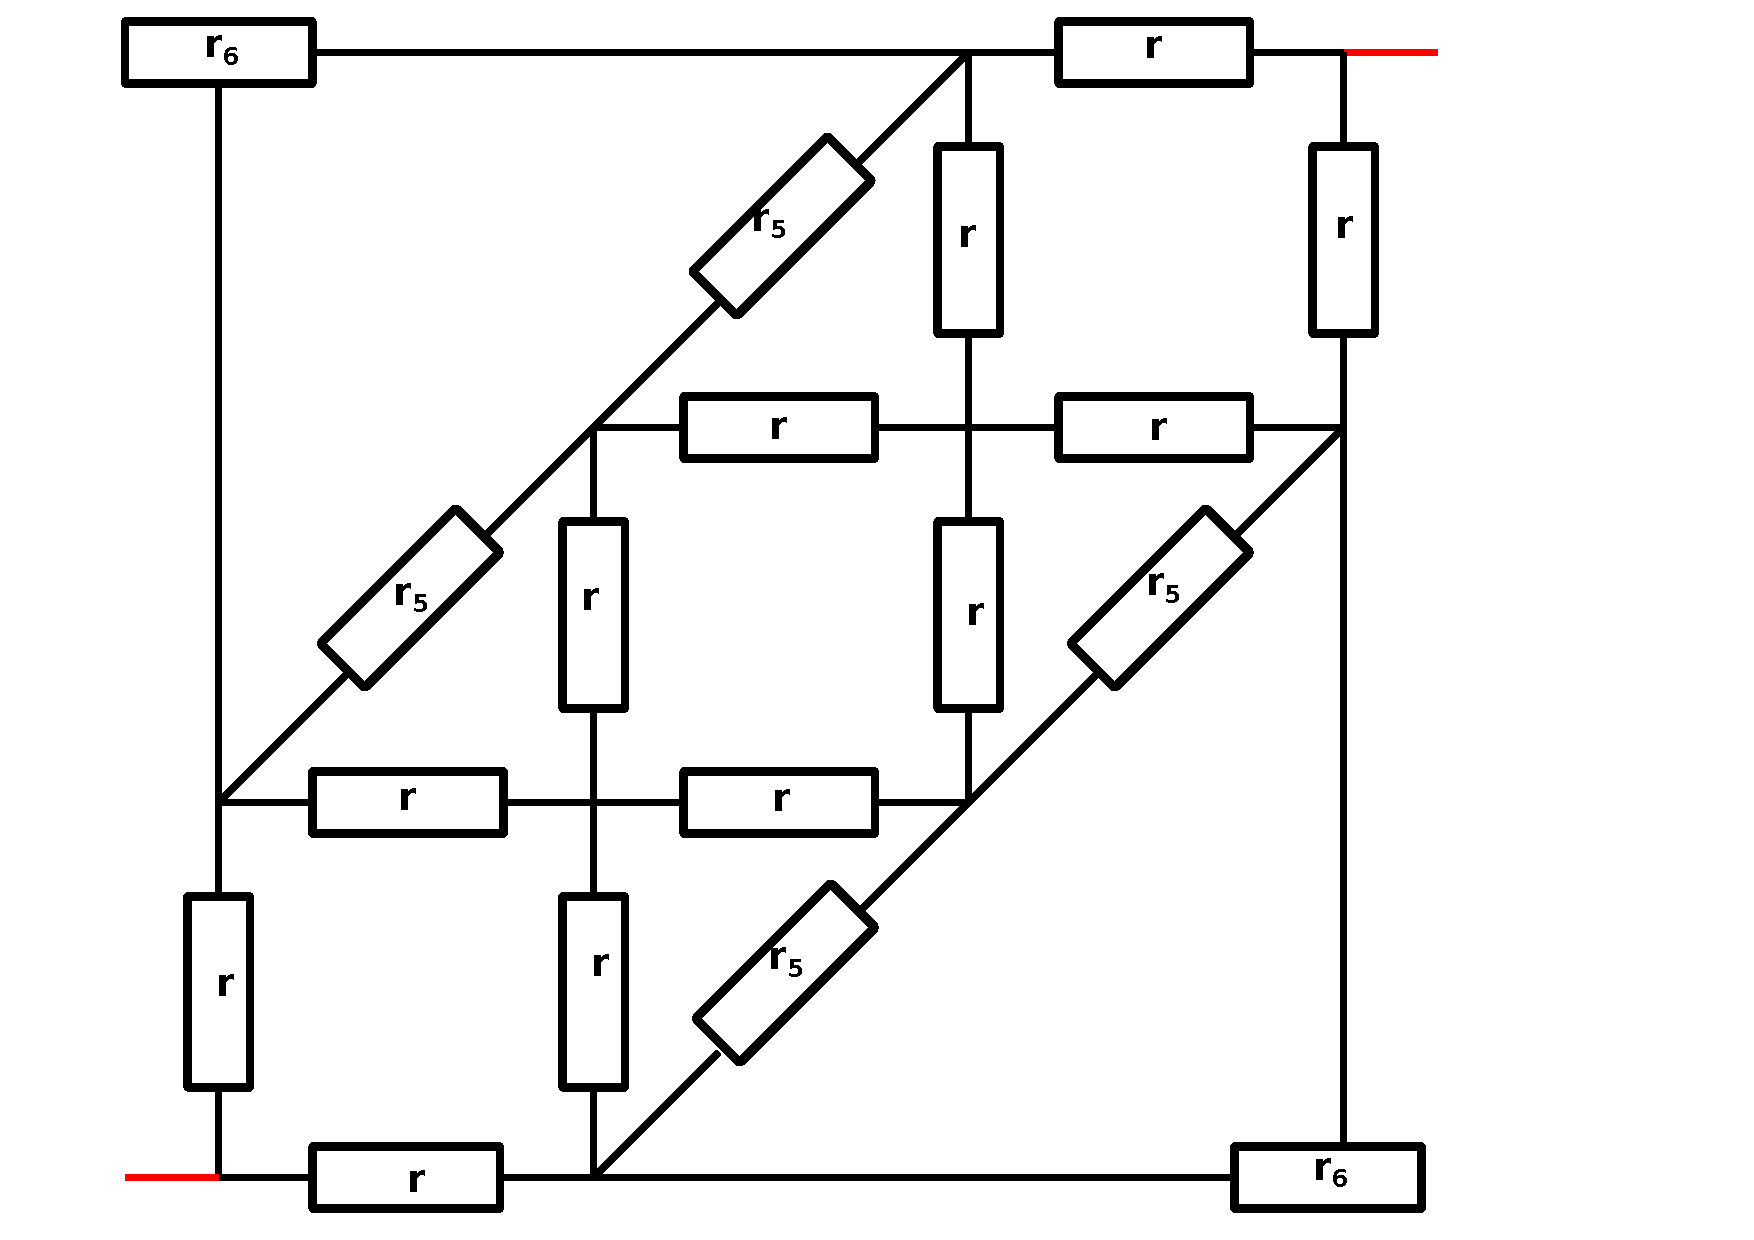
\includegraphics[width=150mm,scale=0.5]{grid_3_4.pdf}
  \caption{Visszaalakítás}
  \label{}
\end{figure}


$$ r_5 = \frac{r_2 \cdot r_3}{r_3} + r_2 + r_3 = 2r $$
$$ r_6 = \frac{r_3 \cdot r_3}{r_2} + r_3 + r_3 = 12r $$
\newpage

Ezeket átalakítva újra soros kapcsolásban lesz négy pár ellenállás. \\
\begin{figure}[h!]
\centering
  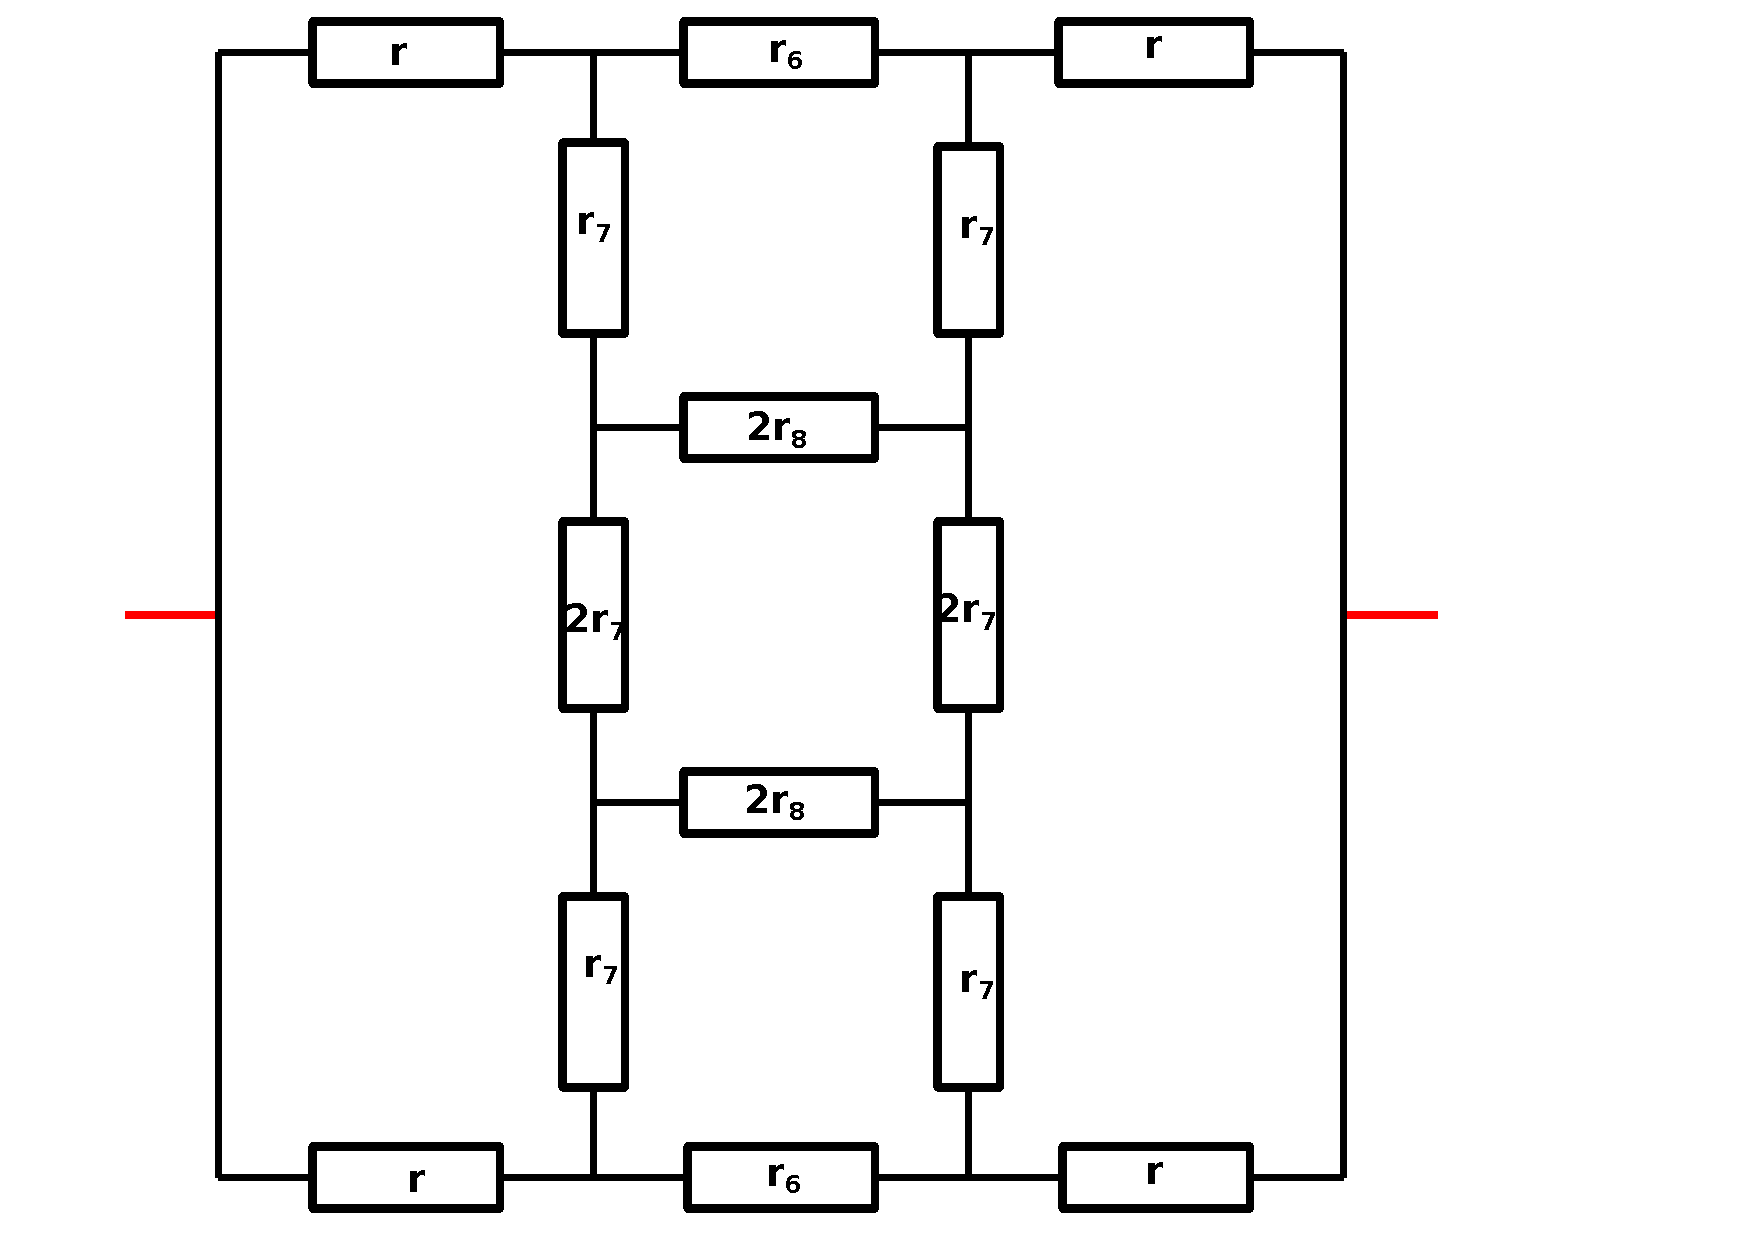
\includegraphics[width=150mm,scale=0.5]{grid_3_5.pdf}
  \caption{Középen lévő csillag-delták átalakítás után}
  \label{}
\end{figure}


$$ r_7 = \frac{r_5 \cdot r}{r + r + r_5} = \frac{1}{2}r $$
$$ r_8 = \frac{r \cdot r}{r + r + r_5} = \frac{1}{4}r $$

\newpage
\indent
A középső négyzet sarkaiaban újabb csillag delták bukkanak fel. Alakítsuk át a bal felső és a jobb alsó sarokban lévőket.Középen megjelenik két ellenállás, melyek párhuzamosan vannak kapcsolva. Ők helyettesíthetők egy ellenállással.\\

\begin{figure}[h!]
\centering
  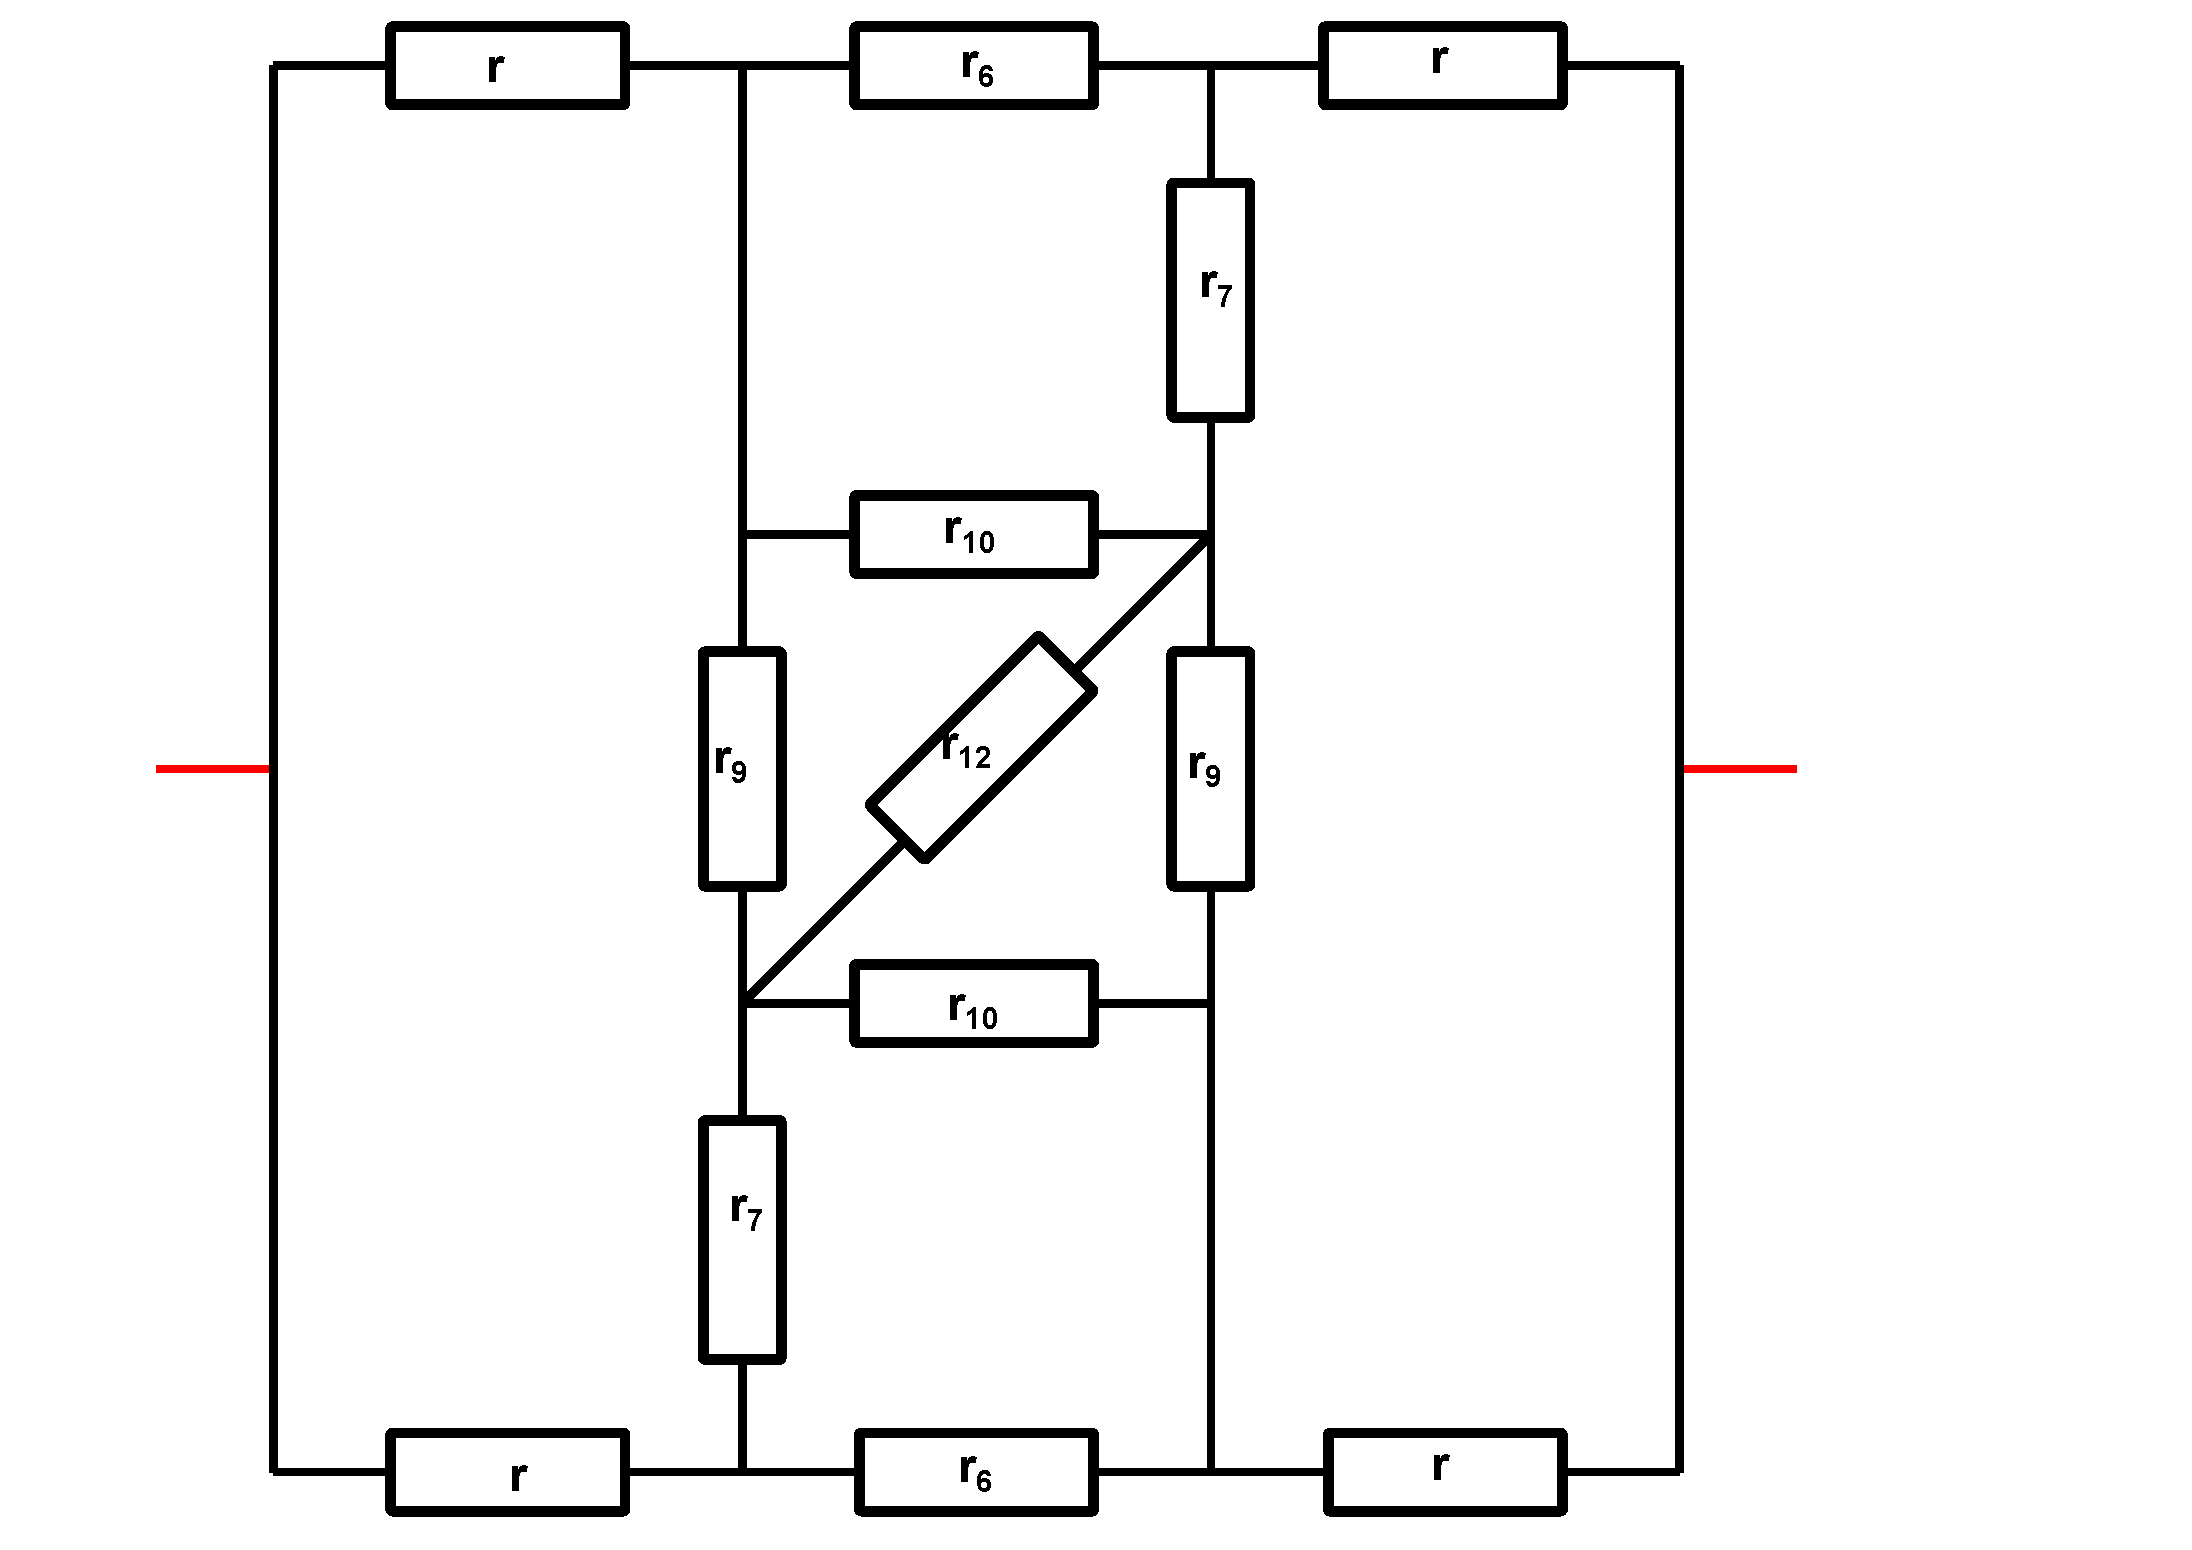
\includegraphics[width=150mm,scale=0.5]{grid_3_6.pdf}
  \caption{}
  \label{}
\end{figure}
$$ r_9 = \frac{r_7 \cdot 2r_7}{2r_8} + r_7 + 2 r_7 = r + \frac{3}{2}r = \frac{5}{2}r $$
$$ r_{10} = \frac{r_7 \cdot 2r_8}{2r_7} + r_7 + 2 r_8 = r $$
$$ r_{11} = \frac{2r_7 \cdot 2r_8}{r_7} + 2 r_7 + 2 r_8 = \frac{5}{2}r $$

$$ \frac{1}{r_{12}} = \frac{2}{r_{11}} $$
$$ r_{12} = \frac{5}{4}r $$

\newpage


A középső négyzet bal felső sarkában és átlójában húzódó háromszöget alakítsuk át.\\

\begin{figure}[h!]
\centering
  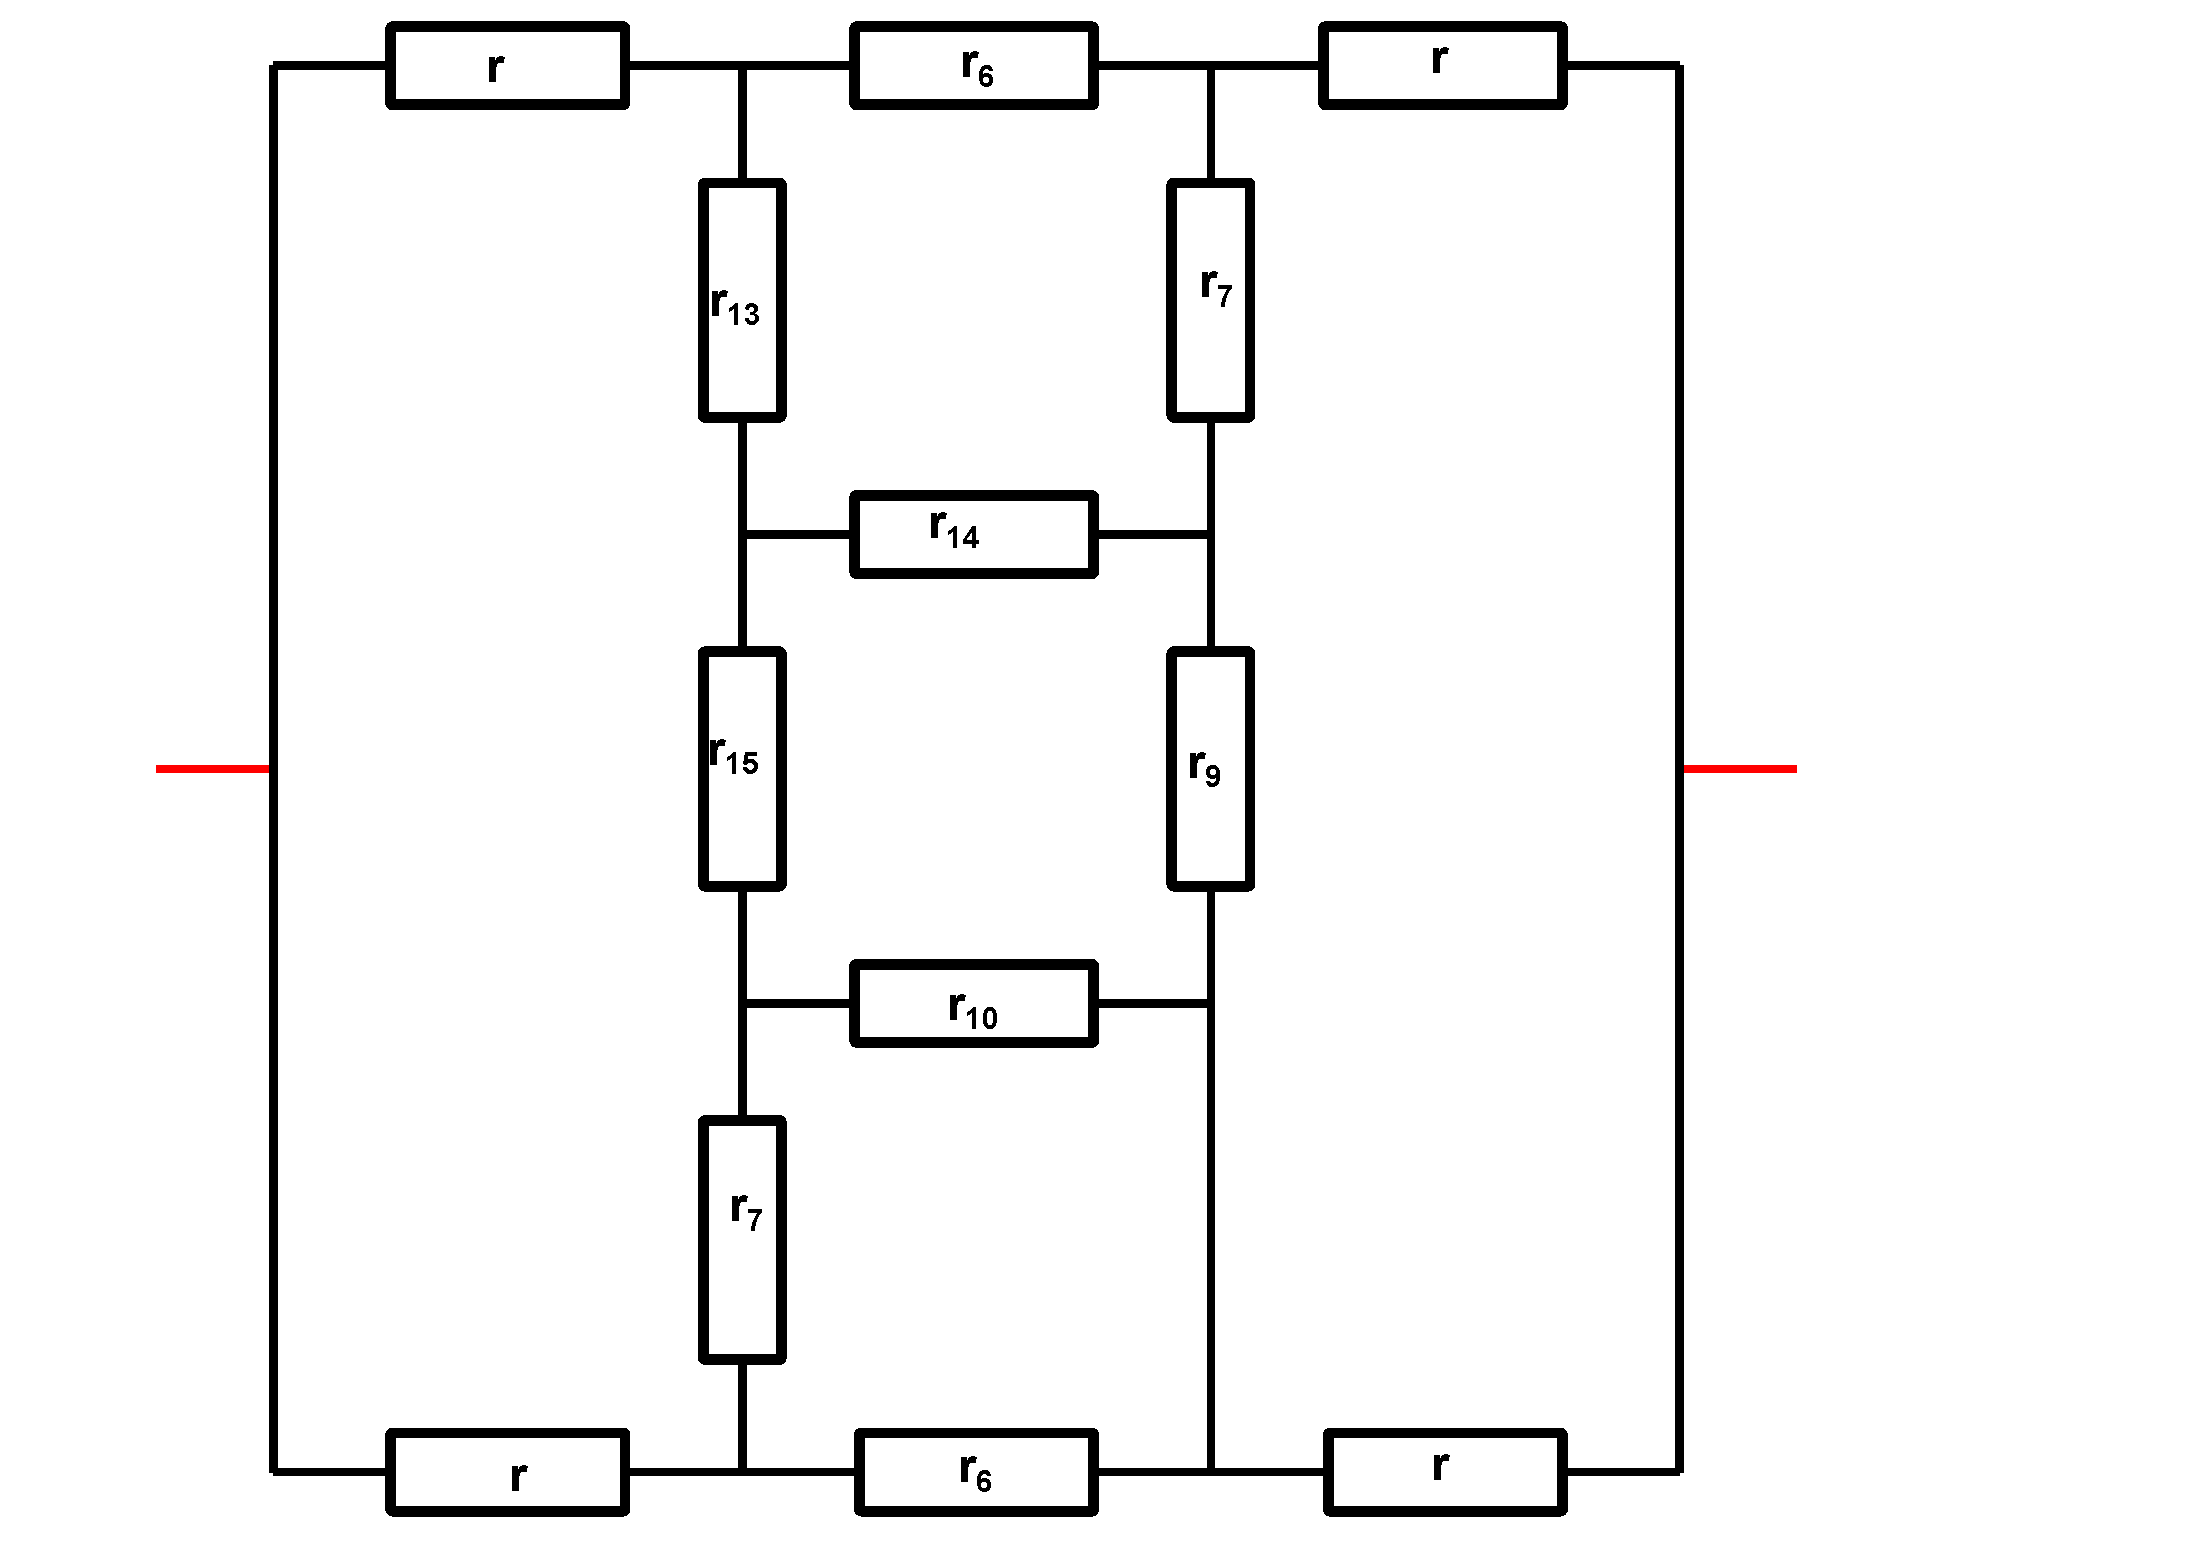
\includegraphics[width=150mm,scale=0.5]{grid_3_7.pdf}
  \caption{}
  \label{}
\end{figure}

$$ r_{13} = \frac{r_9 \cdot r_{10}}{r_9 + r_{10} + r_{12}} = \frac{\frac{5}{2}}{\frac{19}{4}}r = \frac{10}{19} r $$
$$ r_{14} = \frac{r_{10} \cdot r_{12}}{r_9 + r_{10} + r_{12}} = \frac{\frac{9}{4}}{\frac{19}{4}}r = \frac{9}{19} r $$
$$ r_{15} = \frac{r_9 \cdot r_{12}}{r_9 + r_{10} + r_{12}} = \frac{\frac{15}{4}}{\frac{19}{4}}r = \frac{15}{19} r $$



\newpage
A felső négyzet bal felső és jobb alsó sarkát alakítsuk át.\\

\begin{figure}[h!]
\centering
  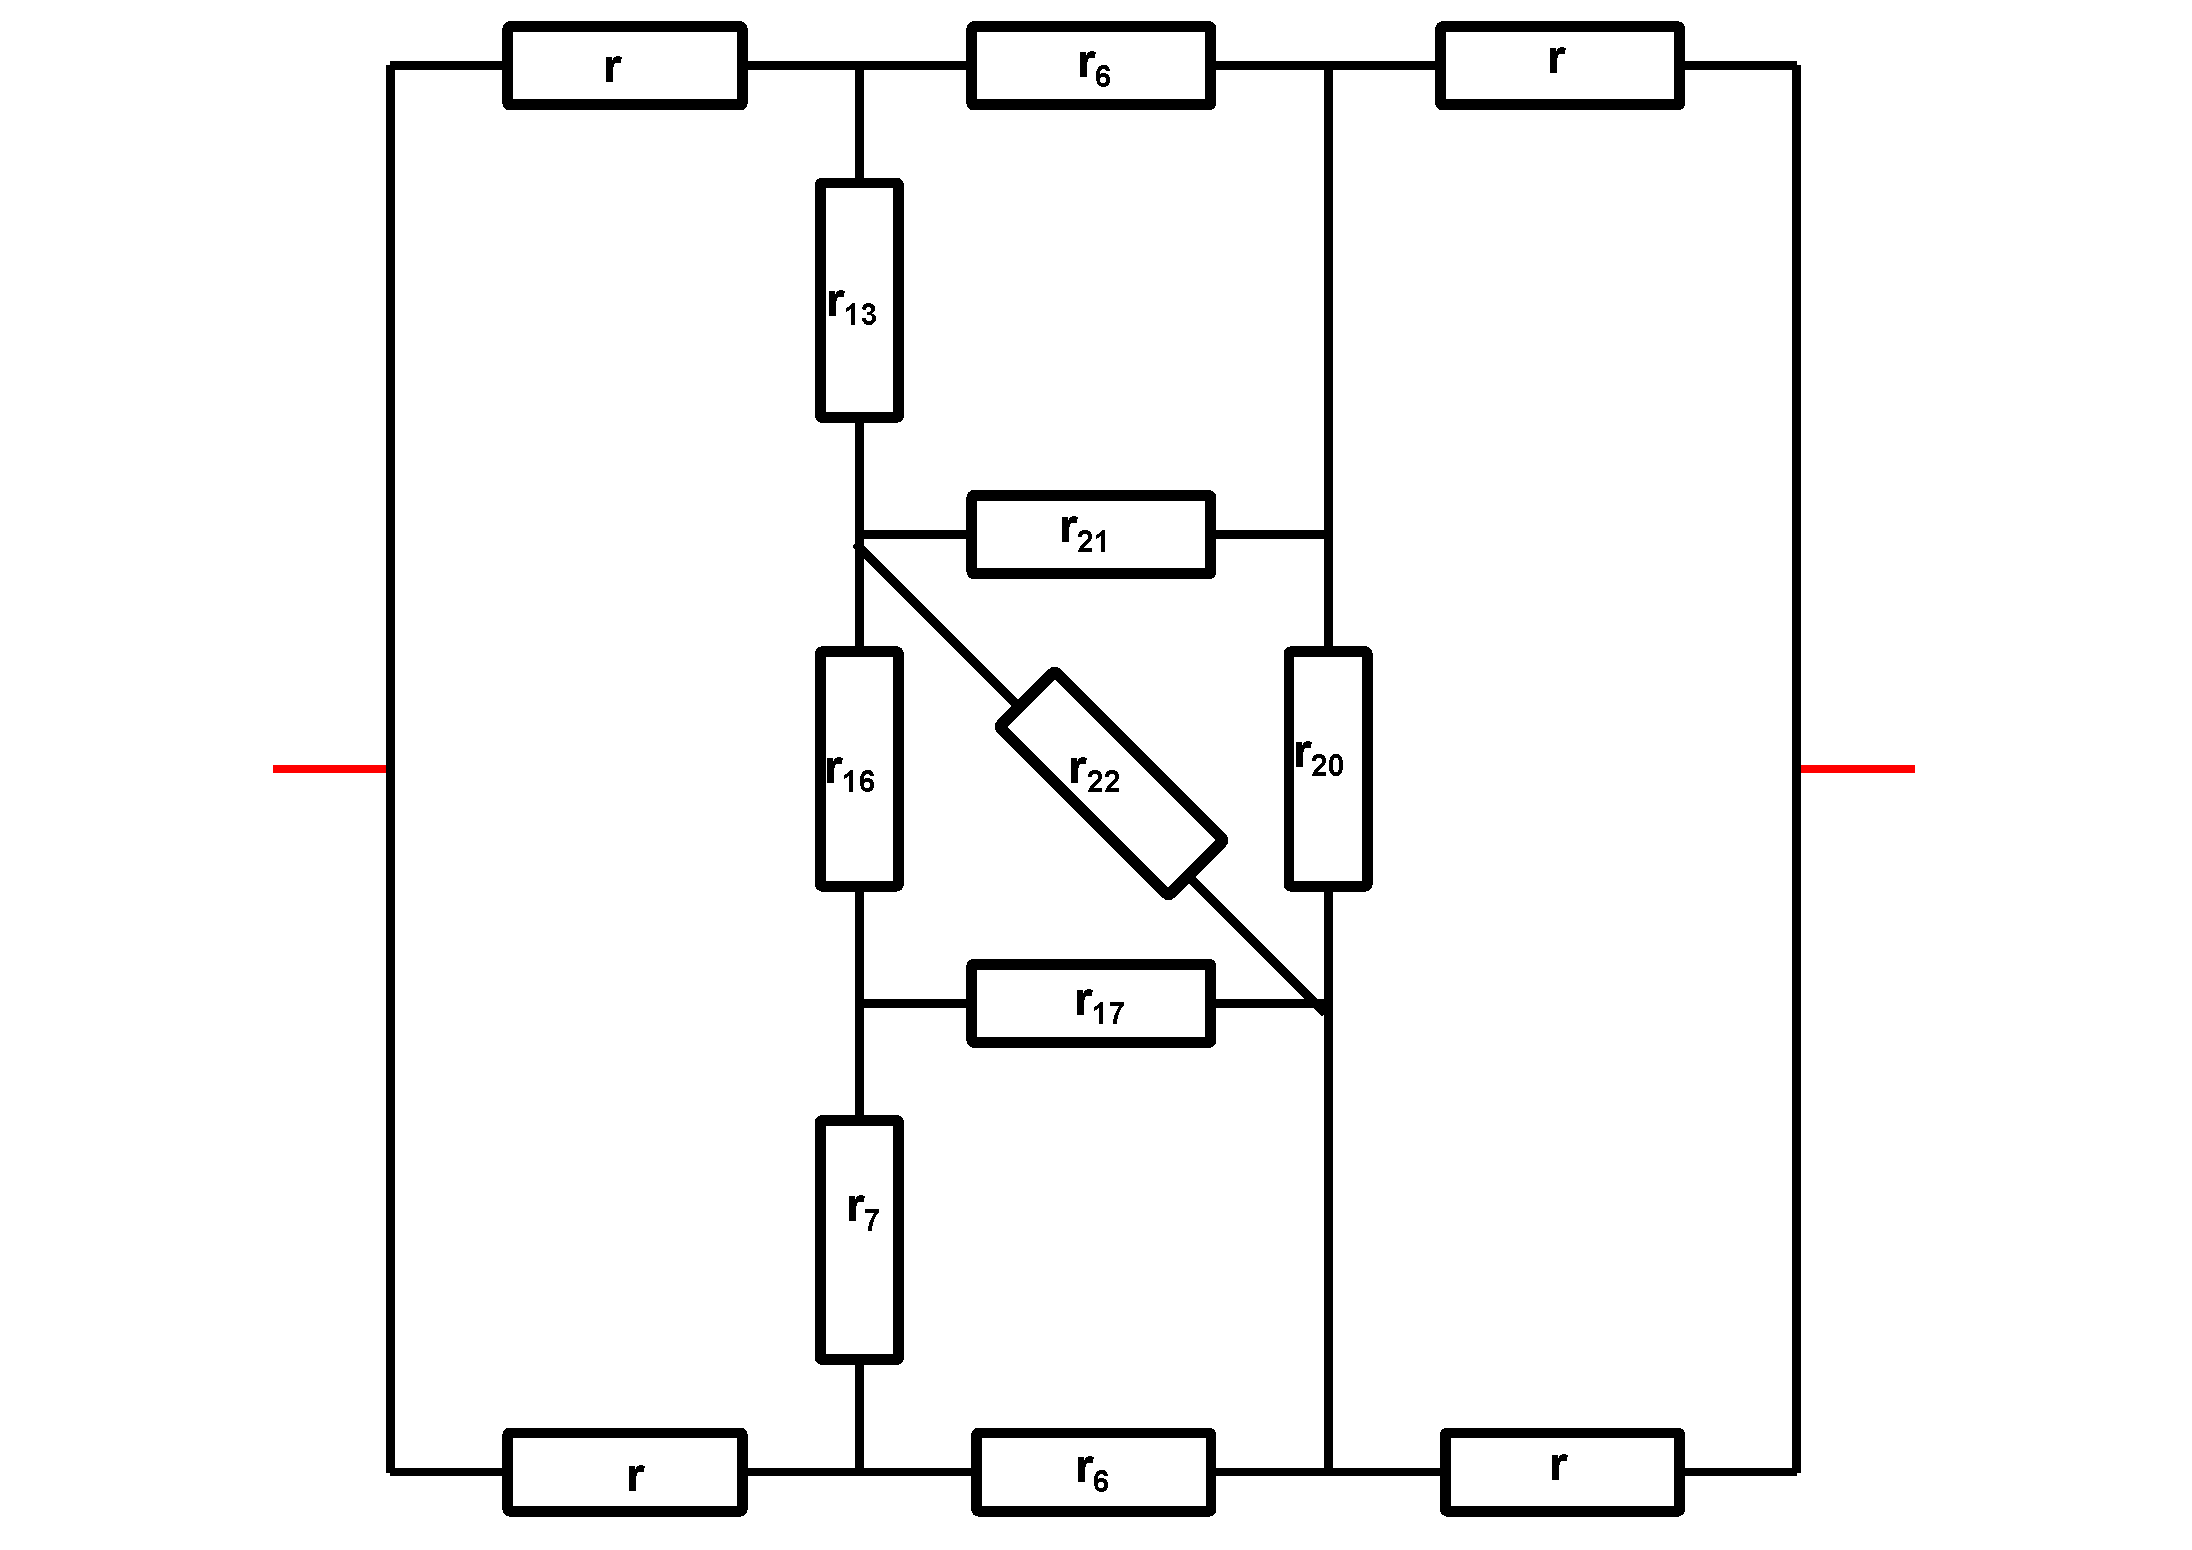
\includegraphics[width=150mm,scale=0.5]{grid_3_8.pdf}
  \caption{}
  \label{}
\end{figure}

$$ r_{16} = \frac{r_7 \cdot r_{15}}{r_{10}} + r_7 + r_{15} = \frac{1}{2} \frac{15}{19}r + \frac{1}{2}r + \frac{15}{19} r = \frac{32}{19} r $$
$$ r_{17} = \frac{r_7 \cdot r_{10}}{r_{15}} + r_7 + r_{10} = \frac{1}{2} \frac{19}{15}r + \frac{1}{2}r + r = \frac{32}{15} r $$
$$ r_{18} = \frac{r_{10} \cdot r_{15}}{r_{7}} + r_{10} + r_{15} = 2 \frac{15}{19}r + r + \frac{15}{19} r = \frac{64}{19} r $$

$$ r_{19} = \frac{r_9 \cdot r_{14}}{r_{7}} + r_9 + r_{14} = 2 \frac{5}{2}r \frac{9}{19}r + \frac{5}{2}r + \frac{9}{19} r  = \frac{79}{19} r $$
$$ r_{20} = \frac{r_7 \cdot r_9}{r_{14}} + r_7 + r_9 = \frac{5}{4} \frac{19}{9}r + \frac{1}{2}r + \frac{5}{2} r = \frac{203}{36} r $$
$$ r_{21} = \frac{r_7 \cdot r_{14}}{r_9} + r_7 + r_{14} = \frac{1}{5} \frac{9}{19}r + \frac{1}{2}r + \frac{9}{19} r = \frac{203}{190} r $$


Újra találkozunk két ellenállással, melyek párhuzamosan vannak kapcsolva.\\
$$ \frac{1}{r_{}22} = \frac{1}{r_{18}} + \frac{1}{r_{19}} =\frac{19}{64r} + \frac{19}{79r} = \frac{2717}{5056r} $$
$$ r_{22} = \frac{2717}{5056}r $$
\newpage
A középső  négyzet jobb felső sarkában és átlójában húzódó delta átalakítható csillaggá.\\

\begin{figure}[h!]
\centering
  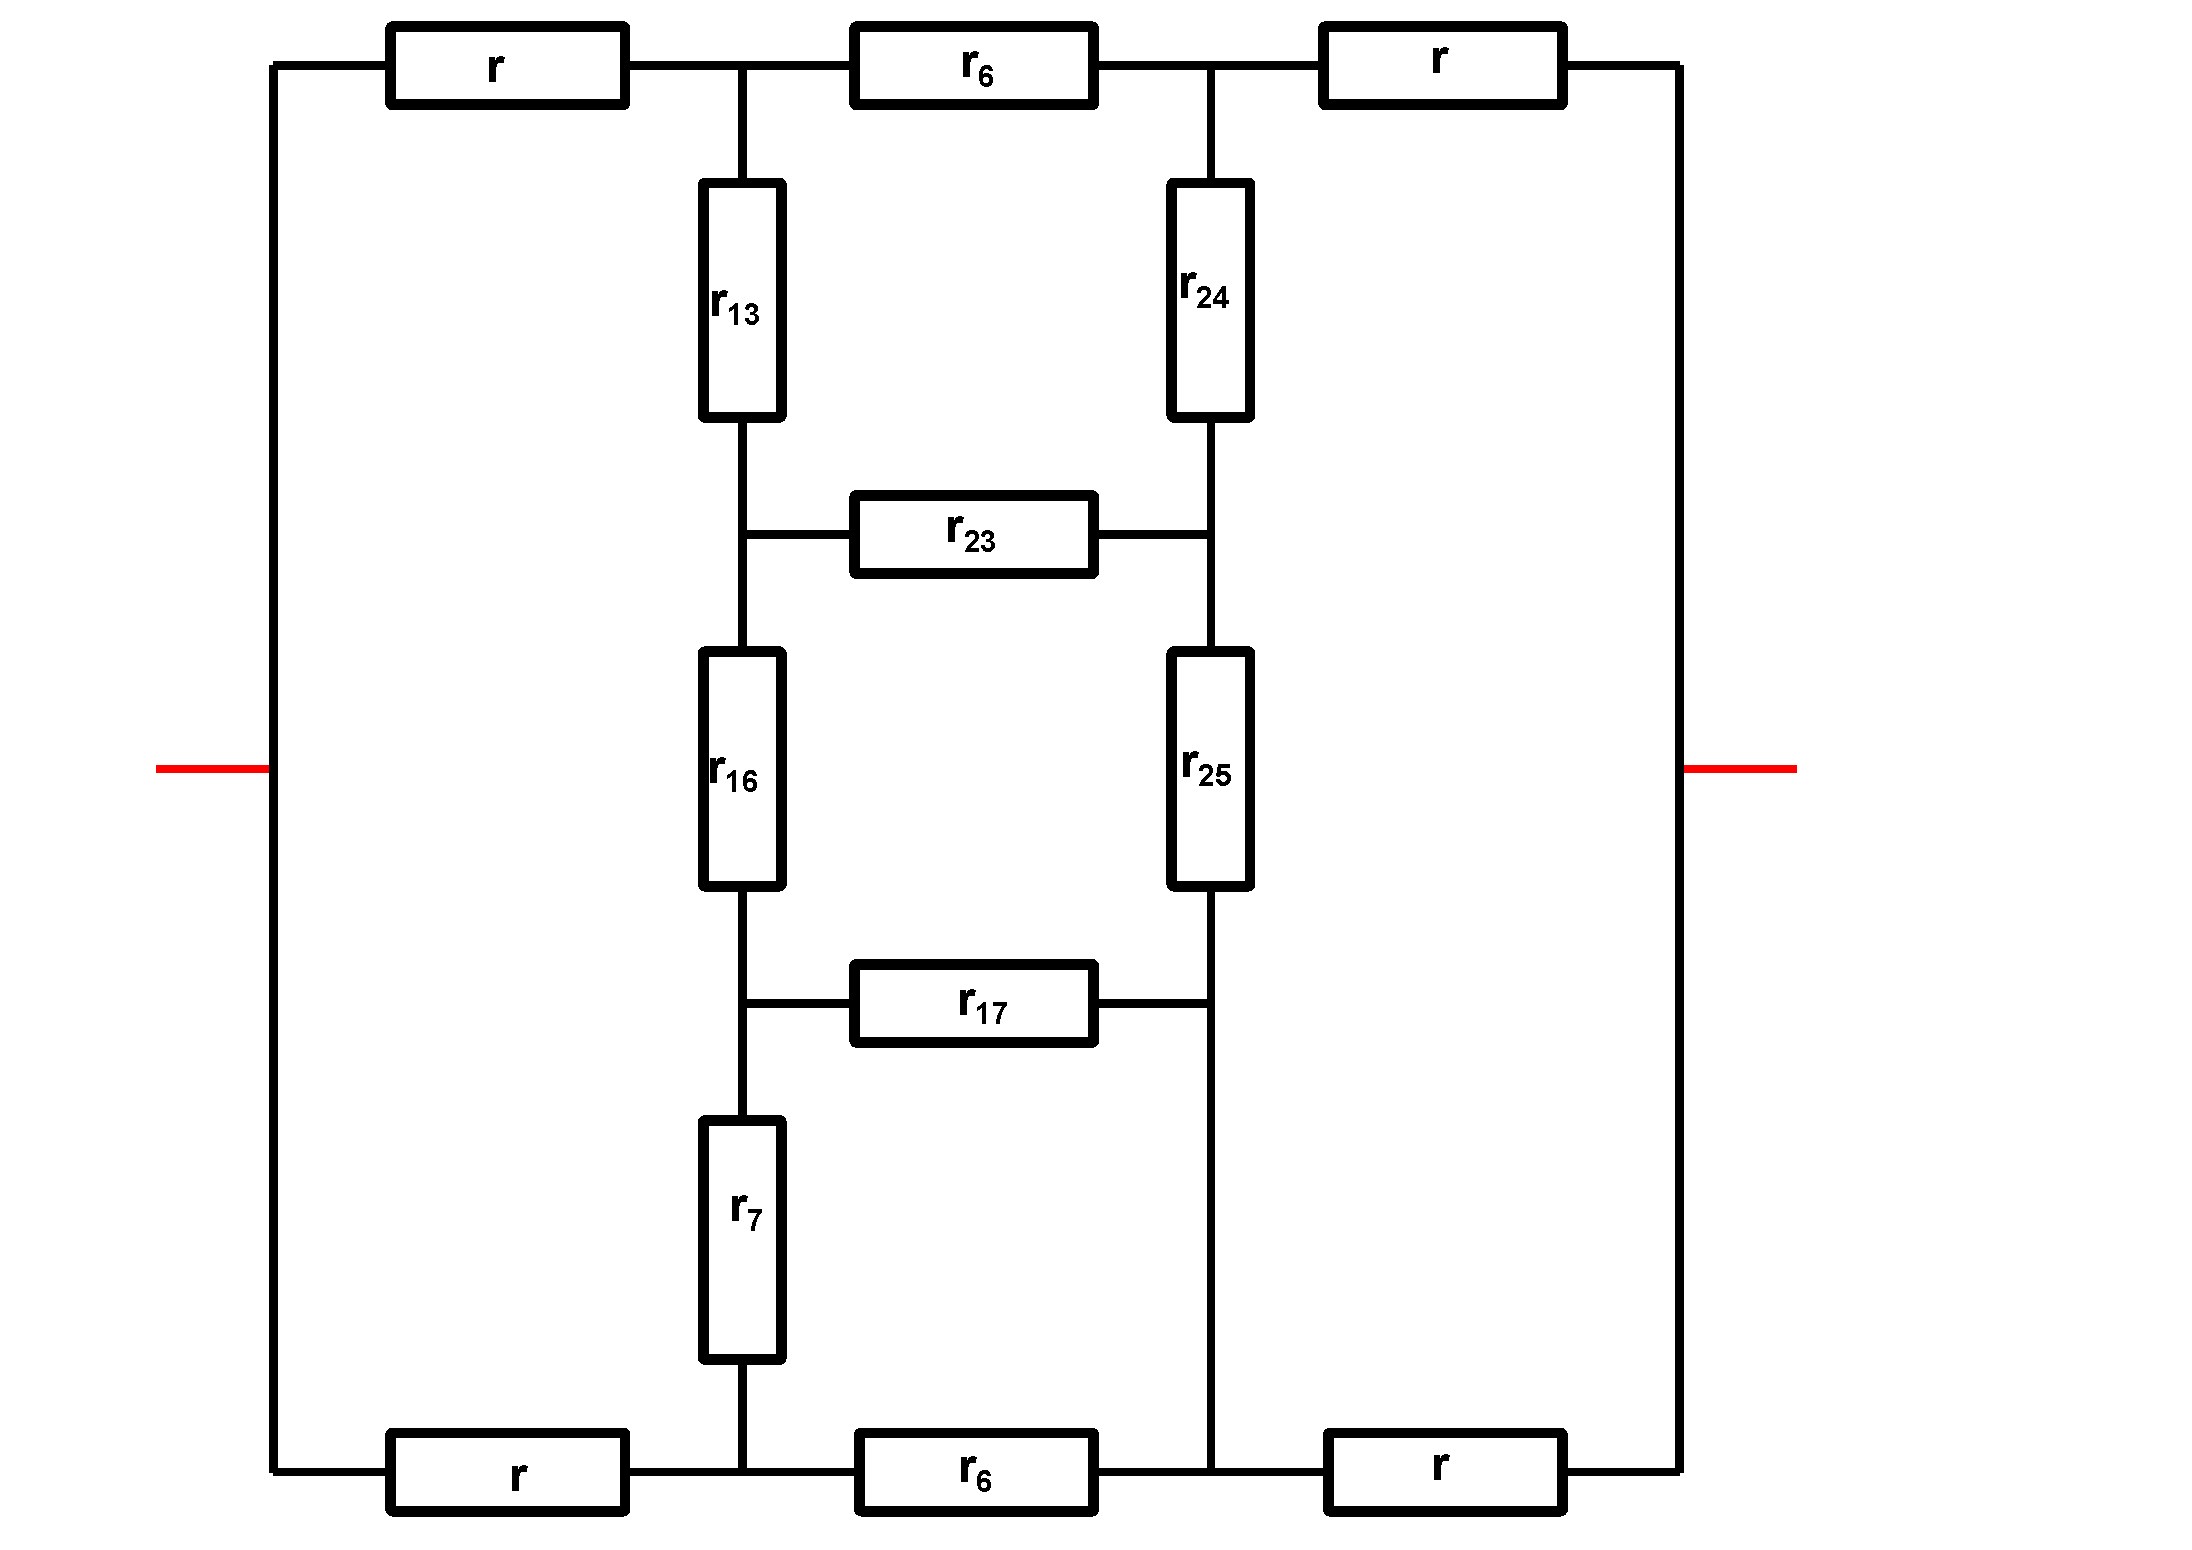
\includegraphics[width=150mm,scale=0.5]{grid_3_9.pdf}
  \caption{}
  \label{}
\end{figure}


$$ r_{23} = \frac{r_{21} \cdot r_{22}}{r_{21} + r_{22} + r_{20}} = \frac{29029}{50560} \cdot \frac{4322880}{5380651}r = \frac{4963959}{10761302}r $$
$$ r_{24} = \frac{r_{21} \cdot r_{20}}{r_{21} + r_{22} + r_{20}} = \frac{41209}{6840} \cdot \frac{4322880}{5380651}r = \frac{26044088}{5380651}$$
$$ r_{25} = \frac{r_{20} \cdot r_{22}}{r_{21} + r_{22} + r_{20}} = \frac{551551}{182016} \cdot \frac{4322880}{5380651}r = \frac{52397345}{21522604}r $$
\newpage
A felső középső négyzet jobb alsó és bal felső sarkába futó csillagok átalakíthatóak deltává. Újabb két párhuzamosan kötött ellenállással találkozunk.\\

\begin{figure}[h!]
\centering
  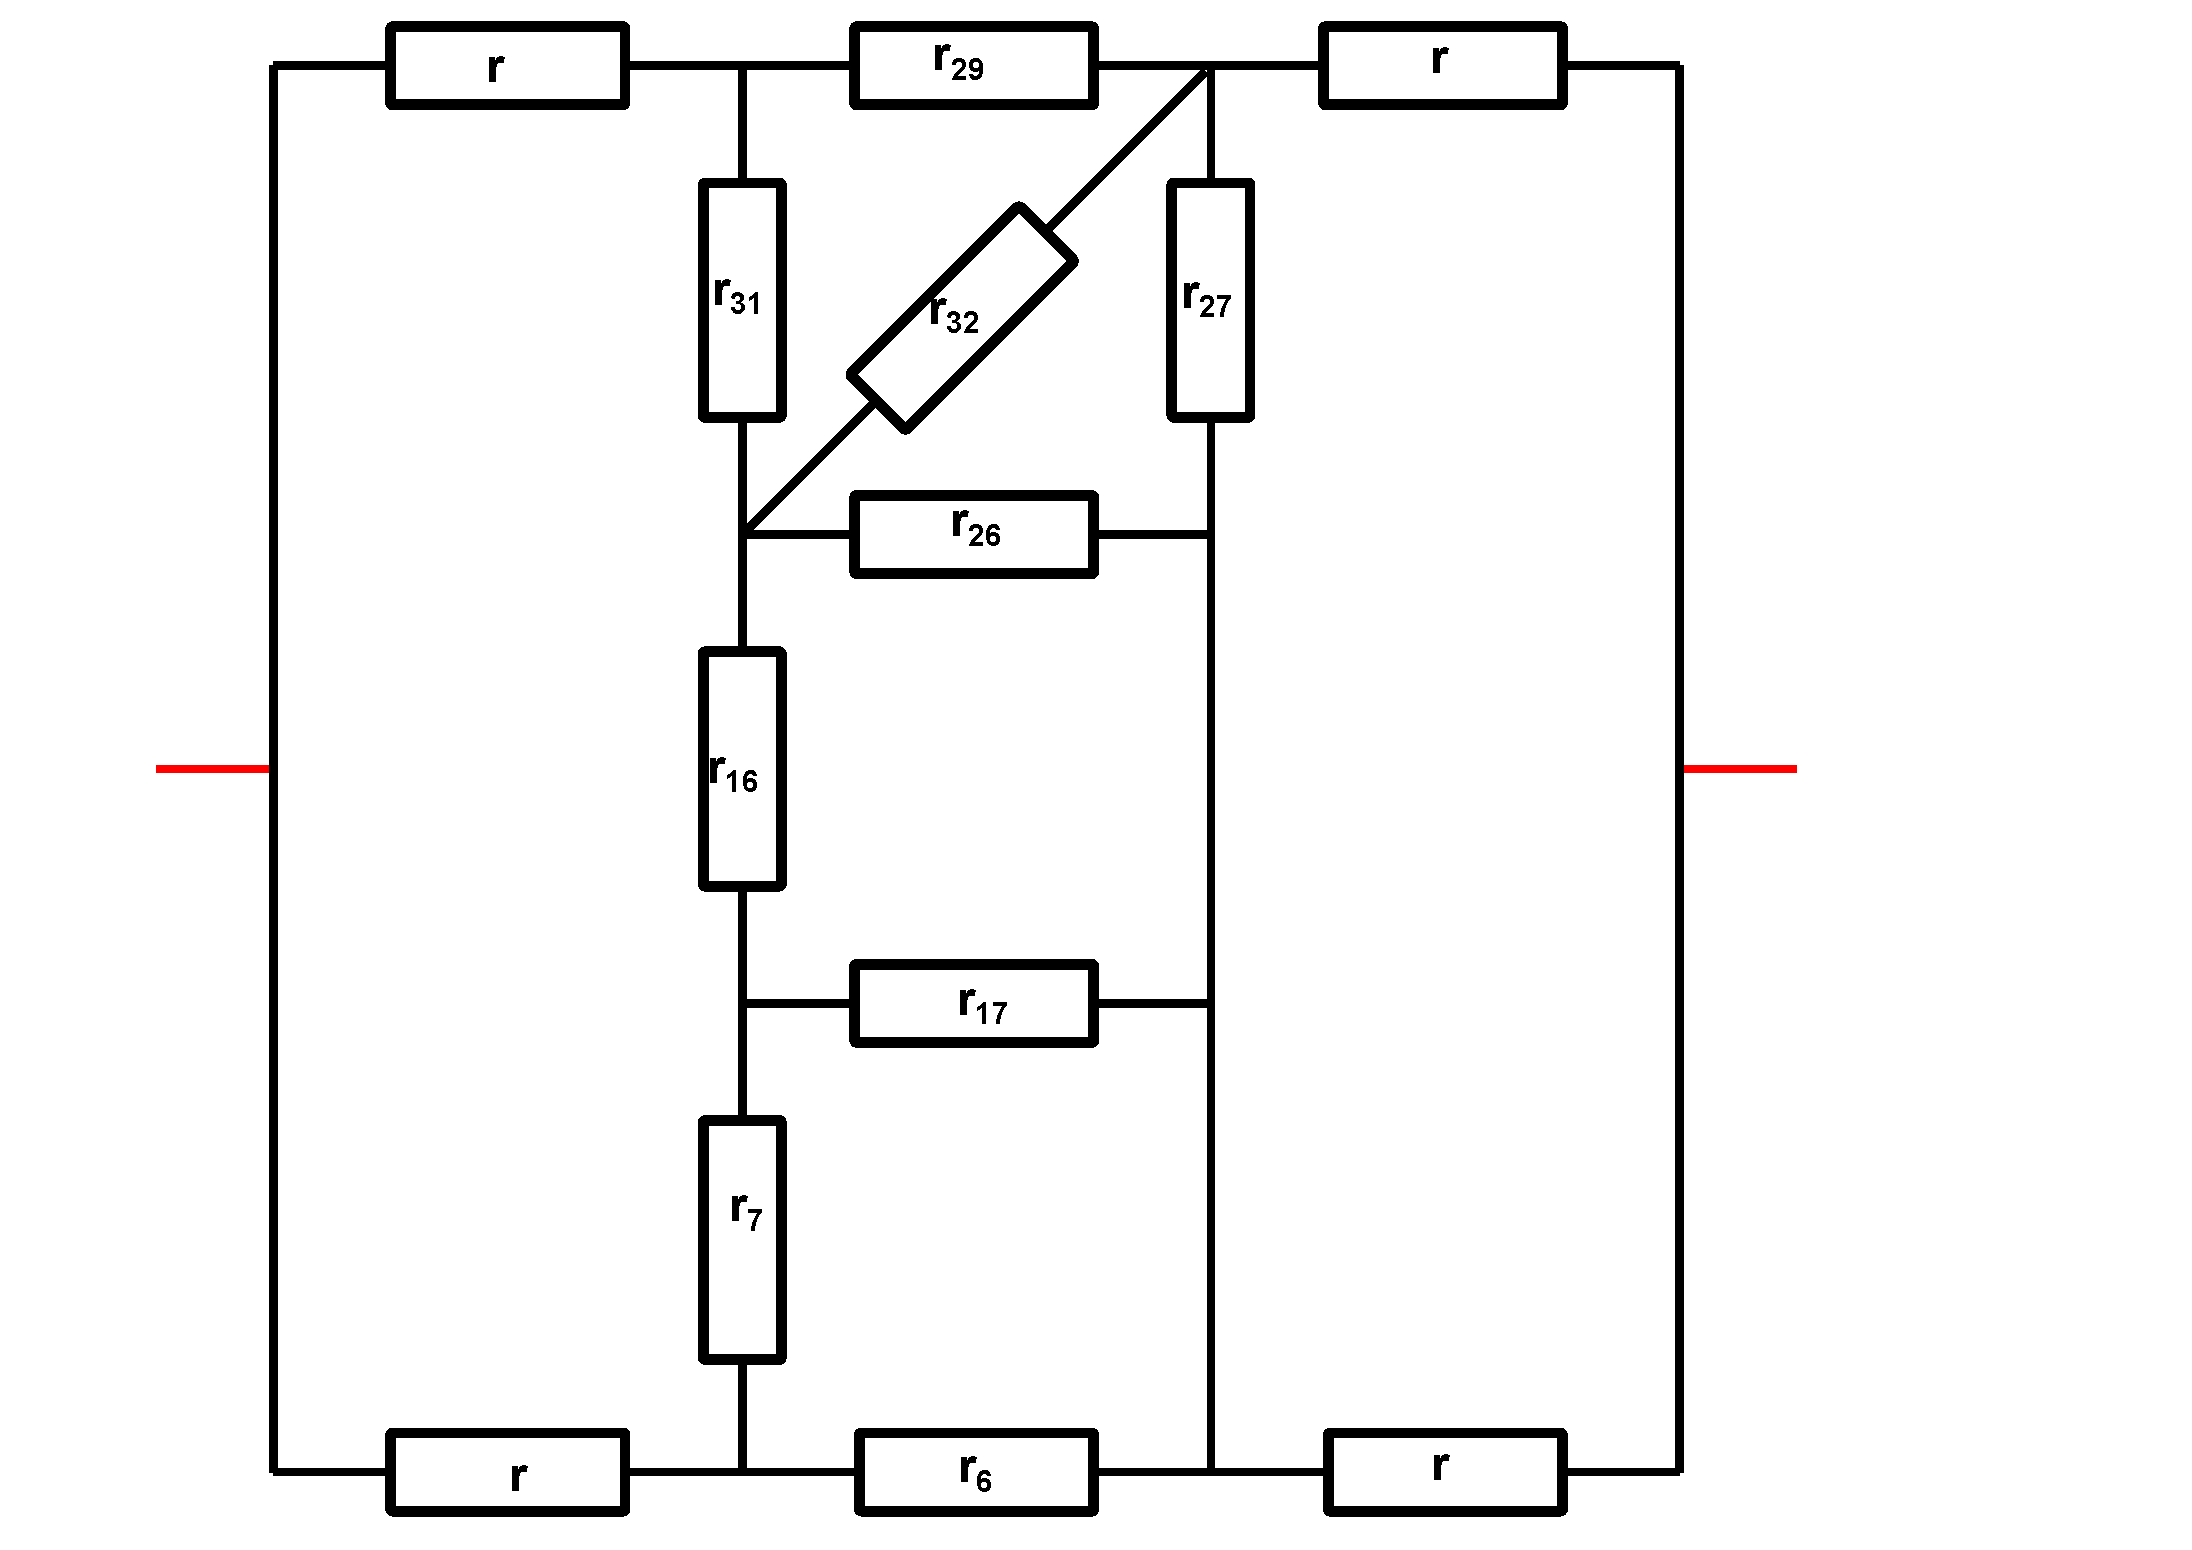
\includegraphics[width=150mm,scale=0.5]{grid_3_10.pdf}
  \caption{}
  \label{}
\end{figure}

Technikai megjegyzés : Sajnos a kalkulátorok nem tudnak több számjegyet befogadni, közelítenek, így kénytelen vagyok tizedes törteket használni. Remélhetőleg a sok tizedes jegy miatt nem lesz akkora hiba a végeredményben.\\
$$ r_{26} = \frac{r_{23} \cdot r_{25}}{r_{24}} + r_{23} + r_{25} = 3,1278132303838633r $$
$$ r_{27} = \frac{r_{24} \cdot r_{25}}{r_{23}} + r_{24} + r_{25} = 32.82099752221226r $$
$$ r_{28} = \frac{r_{24} \cdot r_{23}}{r_{25}} + r_{24} + r_{23} = 6.218715319998111r $$

$$ r_{29} = \frac{r \cdot r_{6}}{r_{13}} + r + r_{6} = 22.75r $$
$$ r_{30} = \frac{r_{13} \cdot r_{6}}{r} + r_{13} + r_{6} = 11.973684210526315r $$
$$ r_{31} = \frac{ \cdot r_{13}}{r_{6}} + r + r_{13} = 1.5964912280701755r $$

$$ \frac{1}{r_{32}} = \frac{1}{r_{28}} + \frac{1}{r_{30}} $$
$$ r_{32} = 4.092969336556398r $$
\newpage
A felső középső négyzet jobb alsó sarkán és átlóján húzódó deltát alakítsuk át csillaggá. \\
Látszik, hogy vannak csomópontok, amik szomszédos csomóponttal ellenállásmentes dróttal vannak összekötve. Ezek ekvipotenciális pontok, úgy is lehet mondani, hogy "összehúzom a két pontot egybe". Ezzel az a technikai nehézség akad, hogy nagyon meggyötört rajzot eredményez.\\ \indent
Ez a lépés több egymás utáni egyszerűsítésre ad lehetőséget, melyek egymásra épülnek. mindezek után egy, az $a)$ feladatból már ismert gráffal találkozunk. Ennek a megoldása az előző feladat végén használt módszerrel gond nélkül kivitelezhető. Tekintve arra, hogy sok hosszú szám és nehezen kifürkészhető képlet vezet a megoldáshoz, a levezetésben jelzem, honnantól analóg a levezetés az előző feladat végével.\\


A deltából csinált csillag ágaiban ezek az ellánállások lesznek:\\
$$ r_{33} = \frac{r_{26} \cdot r_{27}}{r_{32} + r_{27} + r_{26}} = 2.5637708926976983r $$
$$ r_{34} = \frac{r_{32} \cdot r_{27}}{r_{32} + r_{27} + r_{26}} = 3.3548792325044574r $$
$$ r_{35} = \frac{r_{32} \cdot r_{26}}{r_{32} + r_{27} + r_{26}} = 0.3197171457895472r $$ \indent
Az ekvipotenciális csomópontok összekötésével egyértelmű lesz, hogy $r_{16}$ és $r_{17}$ párhuzamosan van kötve:\\
$$ \frac{1}{r_36} = \frac{1}{r_16} + \frac{1}{17} $$
$$ r_{36} = 0.9411764705882353r $$ \indent
Valamint $r_{33}$ és $r_{35}$ is párhuzamosan van kötve:\\
$$ \frac{1}{r_{37}} = \frac{1}{r_{33}} + \frac{1}{{35}} $$
$$ r_{{37}} = 0.2842673530567702r $$ \indent
Ezután $r_{{37}}$ és $r_{{34}}$ sorosan lesz kapcsolva.
$$ r_{{38}} = r_{{37}} + r_{{34}} = 3.6391465855612277r $$ \indent
Valamint $r_{36}$ és $r_6$ párhuzamosan lesz kapcsolva, és az ő eredőjük sorosan $r$-rel.
$$ r_{39} = r + \frac{1}{\frac{1}{r_{36}}+\frac{1}{r_6}} = 1.8362369337979094r $$ \indent
Az $r_{29}$,$r_{31}$ és $r_{38}$ ellenállások egy deltát képeznek, ez átalakítandó csillaggá.\\
$$ r_{40} = \frac{r_{31} \cdot r_{38}}{r_{29} + r_{31} + r_{38}} = 0.20760168627209663r $$
$$ r_{41} = \frac{r_{29} \cdot r_{38}}{r_{29} + r_{31} + r_{38}} = 2.9583240293773767r $$
$$ r_{42} = \frac{r_{29} \cdot r_{31}}{r_{29} + r_{31} + r_{38}} = 1.2978148177457458r $$ \indent
Majd $r_{41}$ és $r$ sorosan lesz kapcsolva, így:
$$ r_{43} = r_{41} + r = 3.9583240293773767r $$
\newpage
\begin{figure}[h!]
\centering
  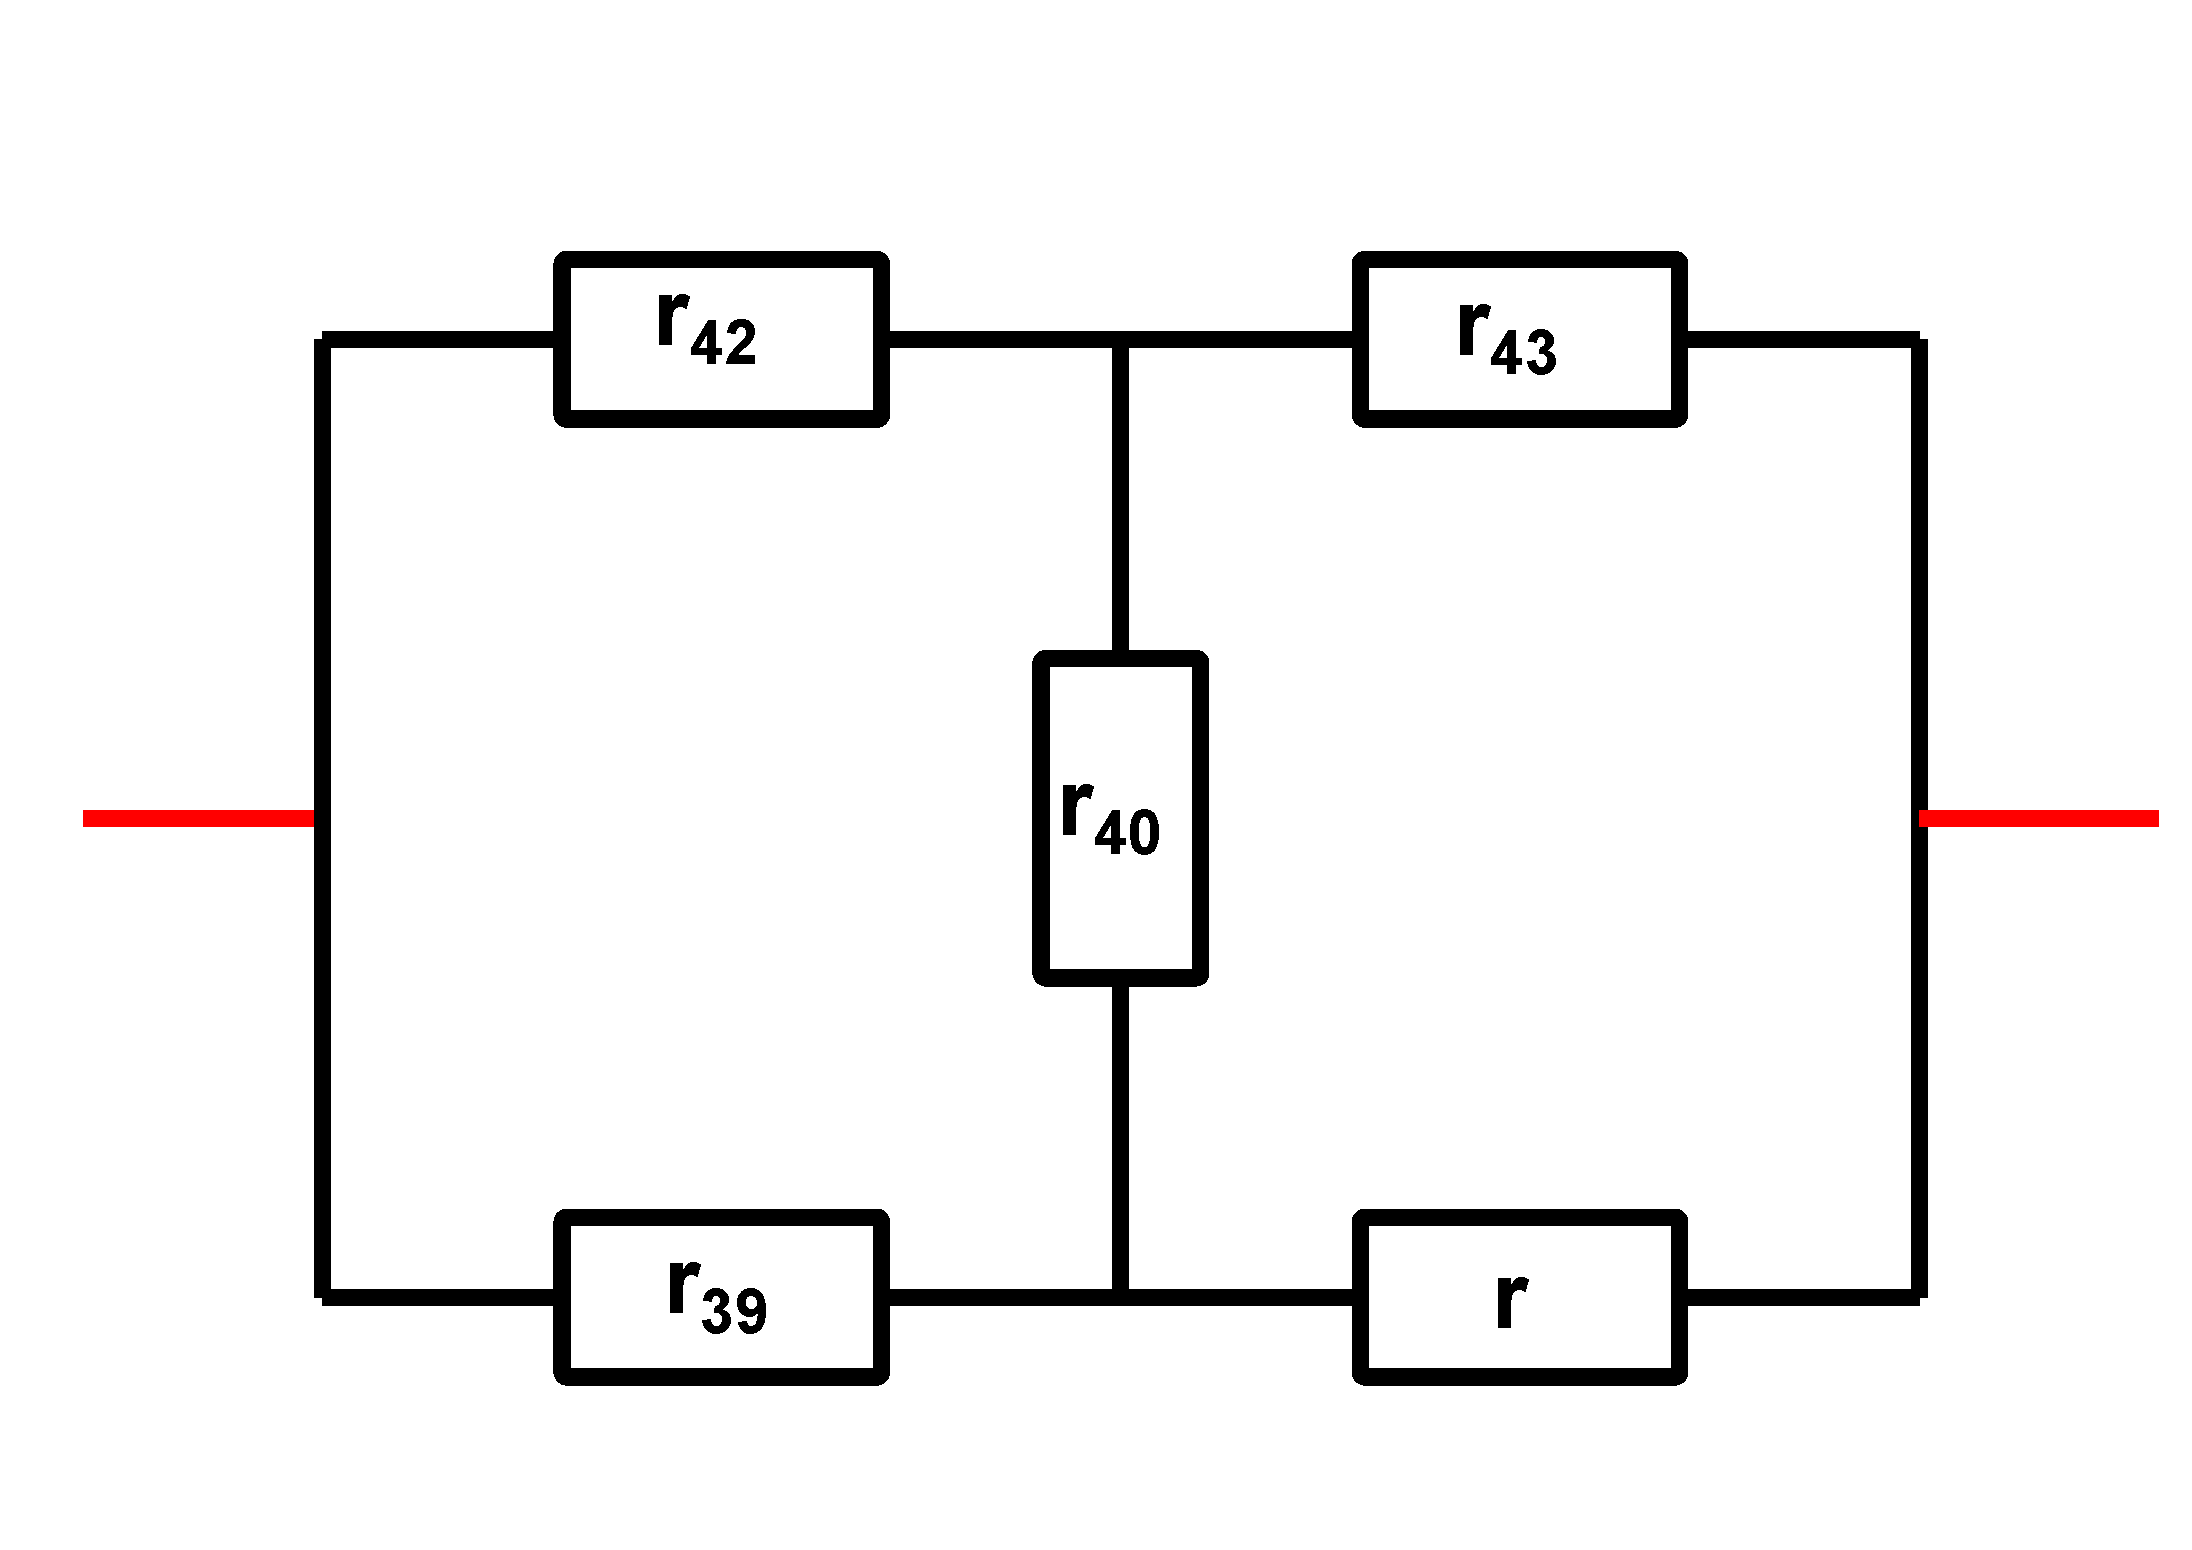
\includegraphics[width=150mm,scale=0.5]{grid_3_11.pdf}
  \caption{}
  \label{}
\end{figure}
\indent

Ez alakra megegyezik az előző feladat végével.\\
A felső kettő és a középső ellenállás átalakítható csillagból deltába.\\
$$ r_{44} = \frac{r_{42} \cdot r_{43}}{r_{40}} + r_{42} + r_{43} = 30.001465684362227r $$
$$ r_{45} = \frac{r_{42} \cdot r_{40}}{r_{43}} + r_{42} + r_{40} = 1.573482822650001r $$
$$ r_{46} = \frac{r_{43} \cdot r_{40}}{r_{42}} + r_{43} + r_{40} = 4.799109072838644r $$ \indent
Itt $r_{45}$ és $r_{39}$ valamint $r_{46}$ és $r$ lesznek párhuzamosan kötve egymás után.
$$ r_{47} = \frac{1}{\frac{1}{r_{45}}+ \frac{1}{r_{39}}} + \frac{1}{\frac{1}{r_{46}}+ \frac{1}{r}} = 1.6749276785069198r $$ \indent
Legeslegvégül pedig $r_{44}$ és $r_{47}$ marad párhuzamosan kapcsolva.
$$ \frac{1}{R} = \frac{1}{r_{44}} + \frac{1}{r_{47}} $$
$$ R = 1.5863638481462r $$






\end{document}